% Chapter 11: Foundation models for time series
% Time Series Analysis -- Bachelor's programmes Economic Informatics and Economic Cybernetics, Bucharest University of Economic Studies
% GENERATED by latex/build_chapter11.py -- edit the generator, not this file.

\newcommand{\coursename}{Time Series Analysis}
% Preambul comun TSA -- Serii de timp / Time Series Analysis (Beamer, 16:9)
% Același design ca MFM și SFM (preluat din SFM, 5 octombrie 2026). Înainte de % Preambul comun TSA -- Serii de timp / Time Series Analysis (Beamer, 16:9)
% Același design ca MFM și SFM (preluat din SFM, 5 octombrie 2026). Înainte de % Preambul comun TSA -- Serii de timp / Time Series Analysis (Beamer, 16:9)
% Același design ca MFM și SFM (preluat din SFM, 5 octombrie 2026). Înainte de \input{../../latex/preamble} se definește
%   \newcommand{\coursename}{Time Series Analysis}      (EN)
%   \newcommand{\coursename}{Serii de timp}       (RO)  și  \def\tsalang{ro}
% Fișierele .tex se află în EN/Courses, EN/Seminars, RO/Cursuri, RO/Seminarii (două niveluri sub rădăcină).
% Deck-urile sînt generate de latex/build_chapterN.py / build_seminarN.py (vezi latex/tsa_build.py).

\documentclass[9pt, aspectratio=169, t]{beamer}
\providecommand{\coursename}{Time Series Analysis}

% Ensure content fits on slides
\setbeamersize{text margin left=8mm, text margin right=8mm}
% Smaller institute font (title page)
\setbeamerfont{institute}{size=\footnotesize}

%=============================================================================
% THEME AND STYLE CONFIGURATION
%=============================================================================
\usetheme{default}
% Using default theme for clean header/footer control

% Color Palette (matching Redispatch PDF)
\definecolor{MainBlue}{RGB}{26, 58, 110}
\definecolor{AccentBlue}{RGB}{26, 58, 110}
\definecolor{IDAred}{RGB}{205, 0, 0}
\definecolor{DarkGray}{RGB}{51, 51, 51}
\definecolor{MediumGray}{RGB}{128, 128, 128}
\definecolor{LightGray}{RGB}{248, 248, 248}
\definecolor{VeryLightGray}{RGB}{235, 235, 235}
\definecolor{KeynoteGray}{RGB}{218, 218, 218}
\definecolor{SectionGray}{RGB}{120, 120, 120}
\definecolor{FooterGray}{RGB}{100, 100, 100}
\definecolor{Crimson}{RGB}{220, 53, 69}
\definecolor{Forest}{RGB}{46, 125, 50}
\definecolor{Amber}{RGB}{181, 133, 63}
\definecolor{Orange}{RGB}{230, 126, 34}
\definecolor{Purple}{RGB}{142, 68, 173}

% Gradient background (exact Keynote 315° gradient: white to RGB 218,218,218)
\setbeamertemplate{background}{%
    \begin{tikzpicture}[remember picture, overlay]
        \shade[shading=axis, shading angle=315,
        top color=white, bottom color=KeynoteGray]
        (current page.south west) rectangle (current page.north east);
    \end{tikzpicture}%
}
% Fallback solid color for compatibility
\setbeamercolor{background canvas}{bg=}

\setbeamercolor{palette primary}{bg=MainBlue, fg=white}
\setbeamercolor{palette secondary}{bg=MainBlue!85, fg=white}
\setbeamercolor{palette tertiary}{bg=MainBlue!70, fg=white}
\setbeamercolor{structure}{fg=MainBlue}
\setbeamercolor{title}{fg=IDAred}
\setbeamercolor{frametitle}{fg=IDAred, bg=}
\setbeamercolor{block title}{bg=MainBlue, fg=white}
\setbeamercolor{block body}{bg=VeryLightGray, fg=DarkGray}
\setbeamercolor{block title alerted}{bg=Crimson, fg=white}
\setbeamercolor{block body alerted}{bg=Crimson!8, fg=DarkGray}
\setbeamercolor{block title example}{bg=Forest, fg=white}
\setbeamercolor{block body example}{bg=Forest!8, fg=DarkGray}
\setbeamercolor{item}{fg=MainBlue}

% Footer colors (override Madrid theme blue)
\setbeamercolor{author in head/foot}{fg=FooterGray, bg=}
\setbeamercolor{title in head/foot}{fg=FooterGray, bg=}
\setbeamercolor{date in head/foot}{fg=FooterGray, bg=}
\setbeamercolor{section in head/foot}{fg=FooterGray, bg=}
\setbeamercolor{subsection in head/foot}{fg=FooterGray, bg=}

% Bullet styles (apply everywhere including blocks)
\setbeamertemplate{itemize item}{\color{MainBlue}$\boxdot$}
\setbeamertemplate{itemize subitem}{\color{MainBlue}$\blacktriangleright$}
\setbeamertemplate{itemize subsubitem}{\color{MainBlue}\tiny$\bullet$}
\setbeamertemplate{itemize/enumerate body begin}{\normalsize}
\setbeamertemplate{itemize/enumerate subbody begin}{\normalsize}

% Item spacing - compact style
\setlength{\leftmargini}{10pt}       % Level 1: minimal indent
\setlength{\leftmarginii}{10pt}      % Level 2: minimal additional indent
% Compact list spacing (zero extra space before/after lists in blocks)
\makeatletter
\def\@listi{\leftmargin\leftmargini \topsep 0pt \parsep 0pt \itemsep 0pt}
\def\@listii{\leftmargin\leftmarginii \topsep 0pt \parsep 0pt \itemsep 0pt}
\makeatother

\setbeamertemplate{navigation symbols}{}

%=============================================================================
% CUSTOM HEADLINE
%=============================================================================
\setbeamertemplate{headline}{%
    \vskip10pt%
    \hbox to \paperwidth{%
        \hskip0.5cm%
        {\small\color{FooterGray}\renewcommand{\hyperlink}[2]{##2}\insertsectionhead}%
        \hfill%
        \textcolor{FooterGray}{\small\insertframenumber}%
        \hskip0.5cm%
    }%
    \vskip4pt%
    {\color{FooterGray}\hrule height 0.4pt}%
}

%=============================================================================
% CUSTOM FOOTER
%=============================================================================
\usepackage{fontawesome5}

\setbeamertemplate{footline}{%
    {\color{FooterGray}\hrule height 0.4pt}%
    \vskip4pt%
    \hbox to \paperwidth{%
        \hskip0.5cm%
        \textcolor{FooterGray}{\small\coursename}%
        \hfill%
        \raisebox{-0.1em}{%
            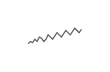
\begin{tikzpicture}[x=0.08em, y=0.08em, line width=0.4pt]
                \draw[FooterGray] (0,3) -- (1,4) -- (2,3.5) -- (3,5) -- (4,4) -- (5,6) -- (6,5.5) -- (7,4) -- (8,5) -- (9,7) -- (10,6) -- (11,5) -- (12,6.5) -- (13,8) -- (14,7) -- (15,6) -- (16,7.5) -- (17,9) -- (18,8) -- (19,7) -- (20,8.5) -- (21,10) -- (22,9) -- (23,8) -- (24,9.5);
            \end{tikzpicture}%
        }%
        \hskip0.5cm%
    }%
    \vskip6pt%
}

%=============================================================================
% PACKAGES
%=============================================================================
\usepackage[utf8]{inputenc}
\DeclareUnicodeCharacter{03B1}{\ensuremath{\alpha}}
\usepackage[T1]{fontenc}
\usepackage{amsmath, amssymb, amsthm}
\usepackage{mathtools}
\usepackage{bm}
\usepackage{tikz}
\usetikzlibrary{arrows.meta, positioning, shapes, calc, decorations.pathreplacing, shadings}
\usepackage{booktabs}
\usepackage{multirow}
\usepackage{array}
\usepackage{graphicx}
\usepackage{animate}
\usepackage{hyperref}
\usepackage{colortbl}
\usepackage{listings}
\lstset{language=Python, basicstyle=\ttfamily\scriptsize, keywordstyle=\color{MainBlue}\bfseries,
  commentstyle=\color{Forest}, stringstyle=\color{Crimson}, breaklines=true,
  frame=none, backgroundcolor=\color{VeryLightGray}, xleftmargin=2mm}
\hypersetup{colorlinks=true, linkcolor=MainBlue, urlcolor=MainBlue}
\graphicspath{{../../logos/}{../../charts/}{../../photos/}}
\usepackage{xcolor}
\hfuzz=2pt  % Suppress tiny overfull warnings (<2pt)
\vfuzz=2pt  % Suppress tiny vertical overfull warnings (<2pt)
% \mathrm in the sans-serif family of the slides (beamer resets \mathrm to the serif family at \begin{document};
% this hook runs after beamer's, so WN, Var, RMSE, ... in formulas match the surrounding text)
% Bold vectors and matrices in the same sans-serif family: \mathbf{A} in sans bold (beamer's own \mathbf came out in
% medium weight), and the bold upright Greek capitals of \boldsymbol / \bm (\bSigma, \bPhi, \boldsymbol{\Theta}) in
% cmss bold: bm.sty fixes its "boldoperators" font when it is loaded (serif cmbx), before beamer switches the
% operators to cmss, so it is reset here.
\AtBeginDocument{%
  \SetMathAlphabet{\mathrm}{normal}{\encodingdefault}{\sfdefault}{\mddefault}{n}%
  \SetMathAlphabet{\mathrm}{bold}{\encodingdefault}{\sfdefault}{bx}{n}%
  \SetMathAlphabet{\mathbf}{normal}{\encodingdefault}{\sfdefault}{bx}{n}%
  \SetMathAlphabet{\mathbf}{bold}{\encodingdefault}{\sfdefault}{bx}{n}%
  \SetSymbolFont{boldoperators}{normal}{OT1}{cmss}{bx}{n}%
  \SetSymbolFont{boldoperators}{bold}{OT1}{cmss}{bx}{n}}

%=============================================================================
% QUANTLET COMMANDS
%   \quantlet{<displayed name>}{<url>}       (generic, compatible with the older TSA decks)
%   \tsaquantlet{Ch_05}{TSA_ch5_garch}       -> https://github.com/danpele/Time-Series-Analysis/tree/main/Quantlets/Ch_05/TSA_ch5_garch
%   \qlurl{<folder>} is defined per chapter by the generator (Quantlets/Ch_NN/<folder>)
%=============================================================================
\newcommand{\tsarepo}{https://github.com/danpele/Time-Series-Analysis}
\newcommand{\tsaqlbase}{https://github.com/danpele/Time-Series-Analysis/tree/main/Quantlets}
\newcommand{\quantlet}[2]{%
    \hfill\href{#2}{%
        \raisebox{-0.15em}{
\includegraphics[height=0.7em]{ql_logo.png}}%
        \textcolor{MainBlue}{\tiny\ #1}%
    }%
}
\newcommand{\tsaquantlet}[2]{\quantlet{\detokenize{#2}}{\tsaqlbase/#1/#2}}

%=============================================================================
% NOTEBOOKS (Google Colab)
%   \colaburl{notebooks/EN/chapter5_seminar_notebook.ipynb} -> the Colab link of a file in the TSA repo
%   \nb: the chapter notebook (each seminar deck redefines it with \renewcommand)
%=============================================================================
\newcommand{\colaburl}[1]{https://colab.research.google.com/github/danpele/Time-Series-Analysis/blob/main/#1}
\newcommand{\nb}{https://colab.research.google.com/github/danpele/Time-Series-Analysis/tree/main/notebooks/EN}
\newcommand{\nbname}{notebooks/EN}

%=============================================================================
% SLIDE HELPERS (used by the generators; the same as in MFM)
%=============================================================================
% local font size for list bodies (the preamble forces \normalsize)
\newcommand{\itemsize}[1]{\setbeamertemplate{itemize/enumerate body begin}{#1}\setbeamertemplate{itemize/enumerate subbody begin}{#1}}
\newcommand{\intitle}[1]{{\hypersetup{urlcolor=white}#1}}   % white links inside coloured title bars
\newcommand{\imgcap}[1]{{\scriptsize #1}\\[0.5mm]}          % caption under a photo
\newcommand{\imgcredit}[2]{{\tiny\color{FooterGray}\href{#1}{#2}}}   % image credit: source URL, author/licence
\newcommand{\aiprompt}[1]{{\ttfamily\color{MainBlue}#1}}     % a prompt to an AI assistant

%=============================================================================
% SEMINARS: student version by default; the instructor wrapper *_solutions.tex sets \solutionstrue
%=============================================================================
\makeatletter\@ifundefined{ifsolutions}{\expandafter\newif\csname ifsolutions\endcsname}{}\makeatother
\newcommand{\solonly}[1]{\ifsolutions #1\fi}
\newcommand{\propsub}{\ifsolutions\else\framesubtitle{\ifdefined\tsalang Rezolvarea se discută la seminar\else Solution discussed in class\fi}\fi}

%=============================================================================
% APPENDIX AND CHAPTER LINKS (latex/appendix_links.py writes the calls; it also re-declares these
% macros before \begin{document}, so the decks compile with or without this preamble block)
%=============================================================================
\providecommand{\tsaapplink}[3]{\hypertarget{#2}{}\hyperlink{#1}{\beamergotobutton{#3}}}
\providecommand{\tsaappback}[2]{\begin{tikzpicture}[remember picture,overlay]\node[anchor=south east] at ([xshift=-3mm,yshift=7mm]current page.south east){\hyperlink{#1}{\beamerreturnbutton{#2}}};\end{tikzpicture}}
\providecommand{\tsachlink}[2]{\href{#1}{#2}}
\providecommand{\tsachlinkt}[2]{\href{#1}{\usebeamercolor[fg]{frametitle}#2}}

%=============================================================================
% QUANTINAR COMMAND: link către un curs Quantinar (subiecte avansate)
%=============================================================================
\newcommand{\quantinar}[2]{%
    \href{#2}{%
        \raisebox{-0.15em}{
\includegraphics[height=0.8em]{qr_logo.png}}%
        \textcolor{MainBlue}{\scriptsize\ #1}%
    }%
}

%=============================================================================
% CUSTOM TITLE PAGE
%=============================================================================
\defbeamertemplate*{title page}{hybrid}[1][]
{
    \vspace{0.2cm}
    % Logos row - top header (with clickable links)
    \begin{center}
        \href{https://www.ase.ro}{
\includegraphics[height=1.0cm]{ase_logo.png}}\hspace{0.3cm}%
        \href{https://theida.net}{
\includegraphics[height=1.0cm]{ida_logo.png}}\hspace{0.3cm}%
        \href{https://blockchain-research-center.com}{
\includegraphics[height=1.0cm]{brc_logo.png}}\hspace{0.3cm}%
        \href{https://www.ai4efin.ase.ro}{
\includegraphics[height=1.0cm]{ai4efin_logo.png}}\hspace{0.3cm}%
        \href{https://ipe.ro/new}{
\includegraphics[height=1.0cm]{acad_logo.png}}\hspace{0.3cm}%
        \href{https://www.digital-finance-msca.com}{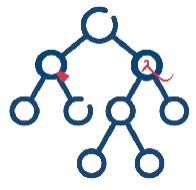
\includegraphics[height=1.0cm]{msca_logo.png}}%
    \end{center}

    \vspace{0.6cm}

    % Main title with Q logos on sides (with clickable links)
    \begin{center}
        \begin{minipage}{0.1\textwidth}
            \centering
            \href{https://quantlet.com}{
\includegraphics[height=1.1cm]{ql_logo.png}}
        \end{minipage}%
        \begin{minipage}{0.78\textwidth}
            \centering
            {\LARGE\bfseries\usebeamercolor[fg]{title}\inserttitle}

            \vspace{0.3cm}

            {\usebeamerfont{subtitle}\usebeamercolor[fg]{title}\insertsubtitle}
        \end{minipage}%
        \begin{minipage}{0.1\textwidth}
            \centering
            \href{https://quantinar.com}{
\includegraphics[height=1.1cm]{qr_logo.png}}
        \end{minipage}
    \end{center}

    \vspace{0.6cm}

    % Authors (left aligned)
    \hspace{0.5cm}{\usebeamerfont{author}\insertauthor}

    \vspace{0.3cm}

    % Institute/Affiliations (left aligned)
    \hspace{0.5cm}\begin{minipage}[t]{0.9\textwidth}
        \raggedright\small\insertinstitute
    \end{minipage}
}

%=============================================================================
% THEOREM ENVIRONMENTS
%=============================================================================
\theoremstyle{definition}
\setbeamertemplate{theorems}[numbered]
\ifdefined\tsalang
\newtheorem{defn}{Definiție}
\newtheorem{thm}{Teoremă}
\newtheorem{prop}{Propoziție}
\newtheorem{rmk}{Observație}
\else
\newtheorem{defn}{Definition}
\newtheorem{thm}{Theorem}
\newtheorem{prop}{Proposition}
\newtheorem{rmk}{Remark}
\fi

%=============================================================================
% CENTRED MINIPAGE (no extra vertical space)
%=============================================================================
\newenvironment{cminipage}[1]{%
    \par\noindent\hfill\begin{minipage}{#1}\ignorespaces
}{%
    \end{minipage}\hfill\null\par
}

%=============================================================================
% CUSTOM COMMANDS
%=============================================================================
\newcommand{\E}{\mathbb{E}}
\newcommand{\Var}{\text{Var}}
\newcommand{\Cov}{\text{Cov}}
\newcommand{\Corr}{\text{Corr}}
\newcommand{\R}{\mathbb{R}}
\newcommand{\N}{\mathbb{N}}
\newcommand{\Z}{\mathbb{Z}}
\newcommand{\B}{\mathbf{B}}
\newcommand{\imark}{\textcolor{MainBlue}{\textbullet}}
\newcommand{\RMSE}{\text{RMSE}}
\newcommand{\MAE}{\text{MAE}}
\newcommand{\MAPE}{\text{MAPE}}

% Boldface vector/matrix commands (VAR, VECM, state space; also used by the older TSA decks)
\newcommand{\bY}{\mathbf{Y}}
\newcommand{\bX}{\mathbf{X}}
\newcommand{\bA}{\mathbf{A}}
\newcommand{\bB}{\mathbf{B}}
\newcommand{\bepsilon}{\boldsymbol{\varepsilon}}
\newcommand{\bSigma}{\boldsymbol{\Sigma}}
\newcommand{\bPhi}{\boldsymbol{\Phi}}
\newcommand{\bGamma}{\boldsymbol{\Gamma}}
\newcommand{\bPi}{\boldsymbol{\Pi}}
\newcommand{\bc}{\mathbf{c}}
\newcommand{\balpha}{\boldsymbol{\alpha}}
\newcommand{\bbeta}{\boldsymbol{\beta}}
\newcommand{\bvarepsilon}{\boldsymbol{\varepsilon}}

% Legacy seminar marks (older TSA seminar decks)
\newcommand{\correct}{\textcolor{Forest}{\checkmark}}
\newcommand{\incorrect}{\textcolor{Crimson}{\texttimes}}
 se definește
%   \newcommand{\coursename}{Time Series Analysis}      (EN)
%   \newcommand{\coursename}{Serii de timp}       (RO)  și  \def\tsalang{ro}
% Fișierele .tex se află în EN/Courses, EN/Seminars, RO/Cursuri, RO/Seminarii (două niveluri sub rădăcină).
% Deck-urile sînt generate de latex/build_chapterN.py / build_seminarN.py (vezi latex/tsa_build.py).

\documentclass[9pt, aspectratio=169, t]{beamer}
\providecommand{\coursename}{Time Series Analysis}

% Ensure content fits on slides
\setbeamersize{text margin left=8mm, text margin right=8mm}
% Smaller institute font (title page)
\setbeamerfont{institute}{size=\footnotesize}

%=============================================================================
% THEME AND STYLE CONFIGURATION
%=============================================================================
\usetheme{default}
% Using default theme for clean header/footer control

% Color Palette (matching Redispatch PDF)
\definecolor{MainBlue}{RGB}{26, 58, 110}
\definecolor{AccentBlue}{RGB}{26, 58, 110}
\definecolor{IDAred}{RGB}{205, 0, 0}
\definecolor{DarkGray}{RGB}{51, 51, 51}
\definecolor{MediumGray}{RGB}{128, 128, 128}
\definecolor{LightGray}{RGB}{248, 248, 248}
\definecolor{VeryLightGray}{RGB}{235, 235, 235}
\definecolor{KeynoteGray}{RGB}{218, 218, 218}
\definecolor{SectionGray}{RGB}{120, 120, 120}
\definecolor{FooterGray}{RGB}{100, 100, 100}
\definecolor{Crimson}{RGB}{220, 53, 69}
\definecolor{Forest}{RGB}{46, 125, 50}
\definecolor{Amber}{RGB}{181, 133, 63}
\definecolor{Orange}{RGB}{230, 126, 34}
\definecolor{Purple}{RGB}{142, 68, 173}

% Gradient background (exact Keynote 315° gradient: white to RGB 218,218,218)
\setbeamertemplate{background}{%
    \begin{tikzpicture}[remember picture, overlay]
        \shade[shading=axis, shading angle=315,
        top color=white, bottom color=KeynoteGray]
        (current page.south west) rectangle (current page.north east);
    \end{tikzpicture}%
}
% Fallback solid color for compatibility
\setbeamercolor{background canvas}{bg=}

\setbeamercolor{palette primary}{bg=MainBlue, fg=white}
\setbeamercolor{palette secondary}{bg=MainBlue!85, fg=white}
\setbeamercolor{palette tertiary}{bg=MainBlue!70, fg=white}
\setbeamercolor{structure}{fg=MainBlue}
\setbeamercolor{title}{fg=IDAred}
\setbeamercolor{frametitle}{fg=IDAred, bg=}
\setbeamercolor{block title}{bg=MainBlue, fg=white}
\setbeamercolor{block body}{bg=VeryLightGray, fg=DarkGray}
\setbeamercolor{block title alerted}{bg=Crimson, fg=white}
\setbeamercolor{block body alerted}{bg=Crimson!8, fg=DarkGray}
\setbeamercolor{block title example}{bg=Forest, fg=white}
\setbeamercolor{block body example}{bg=Forest!8, fg=DarkGray}
\setbeamercolor{item}{fg=MainBlue}

% Footer colors (override Madrid theme blue)
\setbeamercolor{author in head/foot}{fg=FooterGray, bg=}
\setbeamercolor{title in head/foot}{fg=FooterGray, bg=}
\setbeamercolor{date in head/foot}{fg=FooterGray, bg=}
\setbeamercolor{section in head/foot}{fg=FooterGray, bg=}
\setbeamercolor{subsection in head/foot}{fg=FooterGray, bg=}

% Bullet styles (apply everywhere including blocks)
\setbeamertemplate{itemize item}{\color{MainBlue}$\boxdot$}
\setbeamertemplate{itemize subitem}{\color{MainBlue}$\blacktriangleright$}
\setbeamertemplate{itemize subsubitem}{\color{MainBlue}\tiny$\bullet$}
\setbeamertemplate{itemize/enumerate body begin}{\normalsize}
\setbeamertemplate{itemize/enumerate subbody begin}{\normalsize}

% Item spacing - compact style
\setlength{\leftmargini}{10pt}       % Level 1: minimal indent
\setlength{\leftmarginii}{10pt}      % Level 2: minimal additional indent
% Compact list spacing (zero extra space before/after lists in blocks)
\makeatletter
\def\@listi{\leftmargin\leftmargini \topsep 0pt \parsep 0pt \itemsep 0pt}
\def\@listii{\leftmargin\leftmarginii \topsep 0pt \parsep 0pt \itemsep 0pt}
\makeatother

\setbeamertemplate{navigation symbols}{}

%=============================================================================
% CUSTOM HEADLINE
%=============================================================================
\setbeamertemplate{headline}{%
    \vskip10pt%
    \hbox to \paperwidth{%
        \hskip0.5cm%
        {\small\color{FooterGray}\renewcommand{\hyperlink}[2]{##2}\insertsectionhead}%
        \hfill%
        \textcolor{FooterGray}{\small\insertframenumber}%
        \hskip0.5cm%
    }%
    \vskip4pt%
    {\color{FooterGray}\hrule height 0.4pt}%
}

%=============================================================================
% CUSTOM FOOTER
%=============================================================================
\usepackage{fontawesome5}

\setbeamertemplate{footline}{%
    {\color{FooterGray}\hrule height 0.4pt}%
    \vskip4pt%
    \hbox to \paperwidth{%
        \hskip0.5cm%
        \textcolor{FooterGray}{\small\coursename}%
        \hfill%
        \raisebox{-0.1em}{%
            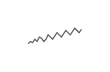
\begin{tikzpicture}[x=0.08em, y=0.08em, line width=0.4pt]
                \draw[FooterGray] (0,3) -- (1,4) -- (2,3.5) -- (3,5) -- (4,4) -- (5,6) -- (6,5.5) -- (7,4) -- (8,5) -- (9,7) -- (10,6) -- (11,5) -- (12,6.5) -- (13,8) -- (14,7) -- (15,6) -- (16,7.5) -- (17,9) -- (18,8) -- (19,7) -- (20,8.5) -- (21,10) -- (22,9) -- (23,8) -- (24,9.5);
            \end{tikzpicture}%
        }%
        \hskip0.5cm%
    }%
    \vskip6pt%
}

%=============================================================================
% PACKAGES
%=============================================================================
\usepackage[utf8]{inputenc}
\DeclareUnicodeCharacter{03B1}{\ensuremath{\alpha}}
\usepackage[T1]{fontenc}
\usepackage{amsmath, amssymb, amsthm}
\usepackage{mathtools}
\usepackage{bm}
\usepackage{tikz}
\usetikzlibrary{arrows.meta, positioning, shapes, calc, decorations.pathreplacing, shadings}
\usepackage{booktabs}
\usepackage{multirow}
\usepackage{array}
\usepackage{graphicx}
\usepackage{animate}
\usepackage{hyperref}
\usepackage{colortbl}
\usepackage{listings}
\lstset{language=Python, basicstyle=\ttfamily\scriptsize, keywordstyle=\color{MainBlue}\bfseries,
  commentstyle=\color{Forest}, stringstyle=\color{Crimson}, breaklines=true,
  frame=none, backgroundcolor=\color{VeryLightGray}, xleftmargin=2mm}
\hypersetup{colorlinks=true, linkcolor=MainBlue, urlcolor=MainBlue}
\graphicspath{{../../logos/}{../../charts/}{../../photos/}}
\usepackage{xcolor}
\hfuzz=2pt  % Suppress tiny overfull warnings (<2pt)
\vfuzz=2pt  % Suppress tiny vertical overfull warnings (<2pt)
% \mathrm in the sans-serif family of the slides (beamer resets \mathrm to the serif family at \begin{document};
% this hook runs after beamer's, so WN, Var, RMSE, ... in formulas match the surrounding text)
% Bold vectors and matrices in the same sans-serif family: \mathbf{A} in sans bold (beamer's own \mathbf came out in
% medium weight), and the bold upright Greek capitals of \boldsymbol / \bm (\bSigma, \bPhi, \boldsymbol{\Theta}) in
% cmss bold: bm.sty fixes its "boldoperators" font when it is loaded (serif cmbx), before beamer switches the
% operators to cmss, so it is reset here.
\AtBeginDocument{%
  \SetMathAlphabet{\mathrm}{normal}{\encodingdefault}{\sfdefault}{\mddefault}{n}%
  \SetMathAlphabet{\mathrm}{bold}{\encodingdefault}{\sfdefault}{bx}{n}%
  \SetMathAlphabet{\mathbf}{normal}{\encodingdefault}{\sfdefault}{bx}{n}%
  \SetMathAlphabet{\mathbf}{bold}{\encodingdefault}{\sfdefault}{bx}{n}%
  \SetSymbolFont{boldoperators}{normal}{OT1}{cmss}{bx}{n}%
  \SetSymbolFont{boldoperators}{bold}{OT1}{cmss}{bx}{n}}

%=============================================================================
% QUANTLET COMMANDS
%   \quantlet{<displayed name>}{<url>}       (generic, compatible with the older TSA decks)
%   \tsaquantlet{Ch_05}{TSA_ch5_garch}       -> https://github.com/danpele/Time-Series-Analysis/tree/main/Quantlets/Ch_05/TSA_ch5_garch
%   \qlurl{<folder>} is defined per chapter by the generator (Quantlets/Ch_NN/<folder>)
%=============================================================================
\newcommand{\tsarepo}{https://github.com/danpele/Time-Series-Analysis}
\newcommand{\tsaqlbase}{https://github.com/danpele/Time-Series-Analysis/tree/main/Quantlets}
\newcommand{\quantlet}[2]{%
    \hfill\href{#2}{%
        \raisebox{-0.15em}{
\includegraphics[height=0.7em]{ql_logo.png}}%
        \textcolor{MainBlue}{\tiny\ #1}%
    }%
}
\newcommand{\tsaquantlet}[2]{\quantlet{\detokenize{#2}}{\tsaqlbase/#1/#2}}

%=============================================================================
% NOTEBOOKS (Google Colab)
%   \colaburl{notebooks/EN/chapter5_seminar_notebook.ipynb} -> the Colab link of a file in the TSA repo
%   \nb: the chapter notebook (each seminar deck redefines it with \renewcommand)
%=============================================================================
\newcommand{\colaburl}[1]{https://colab.research.google.com/github/danpele/Time-Series-Analysis/blob/main/#1}
\newcommand{\nb}{https://colab.research.google.com/github/danpele/Time-Series-Analysis/tree/main/notebooks/EN}
\newcommand{\nbname}{notebooks/EN}

%=============================================================================
% SLIDE HELPERS (used by the generators; the same as in MFM)
%=============================================================================
% local font size for list bodies (the preamble forces \normalsize)
\newcommand{\itemsize}[1]{\setbeamertemplate{itemize/enumerate body begin}{#1}\setbeamertemplate{itemize/enumerate subbody begin}{#1}}
\newcommand{\intitle}[1]{{\hypersetup{urlcolor=white}#1}}   % white links inside coloured title bars
\newcommand{\imgcap}[1]{{\scriptsize #1}\\[0.5mm]}          % caption under a photo
\newcommand{\imgcredit}[2]{{\tiny\color{FooterGray}\href{#1}{#2}}}   % image credit: source URL, author/licence
\newcommand{\aiprompt}[1]{{\ttfamily\color{MainBlue}#1}}     % a prompt to an AI assistant

%=============================================================================
% SEMINARS: student version by default; the instructor wrapper *_solutions.tex sets \solutionstrue
%=============================================================================
\makeatletter\@ifundefined{ifsolutions}{\expandafter\newif\csname ifsolutions\endcsname}{}\makeatother
\newcommand{\solonly}[1]{\ifsolutions #1\fi}
\newcommand{\propsub}{\ifsolutions\else\framesubtitle{\ifdefined\tsalang Rezolvarea se discută la seminar\else Solution discussed in class\fi}\fi}

%=============================================================================
% APPENDIX AND CHAPTER LINKS (latex/appendix_links.py writes the calls; it also re-declares these
% macros before \begin{document}, so the decks compile with or without this preamble block)
%=============================================================================
\providecommand{\tsaapplink}[3]{\hypertarget{#2}{}\hyperlink{#1}{\beamergotobutton{#3}}}
\providecommand{\tsaappback}[2]{\begin{tikzpicture}[remember picture,overlay]\node[anchor=south east] at ([xshift=-3mm,yshift=7mm]current page.south east){\hyperlink{#1}{\beamerreturnbutton{#2}}};\end{tikzpicture}}
\providecommand{\tsachlink}[2]{\href{#1}{#2}}
\providecommand{\tsachlinkt}[2]{\href{#1}{\usebeamercolor[fg]{frametitle}#2}}

%=============================================================================
% QUANTINAR COMMAND: link către un curs Quantinar (subiecte avansate)
%=============================================================================
\newcommand{\quantinar}[2]{%
    \href{#2}{%
        \raisebox{-0.15em}{
\includegraphics[height=0.8em]{qr_logo.png}}%
        \textcolor{MainBlue}{\scriptsize\ #1}%
    }%
}

%=============================================================================
% CUSTOM TITLE PAGE
%=============================================================================
\defbeamertemplate*{title page}{hybrid}[1][]
{
    \vspace{0.2cm}
    % Logos row - top header (with clickable links)
    \begin{center}
        \href{https://www.ase.ro}{
\includegraphics[height=1.0cm]{ase_logo.png}}\hspace{0.3cm}%
        \href{https://theida.net}{
\includegraphics[height=1.0cm]{ida_logo.png}}\hspace{0.3cm}%
        \href{https://blockchain-research-center.com}{
\includegraphics[height=1.0cm]{brc_logo.png}}\hspace{0.3cm}%
        \href{https://www.ai4efin.ase.ro}{
\includegraphics[height=1.0cm]{ai4efin_logo.png}}\hspace{0.3cm}%
        \href{https://ipe.ro/new}{
\includegraphics[height=1.0cm]{acad_logo.png}}\hspace{0.3cm}%
        \href{https://www.digital-finance-msca.com}{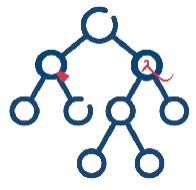
\includegraphics[height=1.0cm]{msca_logo.png}}%
    \end{center}

    \vspace{0.6cm}

    % Main title with Q logos on sides (with clickable links)
    \begin{center}
        \begin{minipage}{0.1\textwidth}
            \centering
            \href{https://quantlet.com}{
\includegraphics[height=1.1cm]{ql_logo.png}}
        \end{minipage}%
        \begin{minipage}{0.78\textwidth}
            \centering
            {\LARGE\bfseries\usebeamercolor[fg]{title}\inserttitle}

            \vspace{0.3cm}

            {\usebeamerfont{subtitle}\usebeamercolor[fg]{title}\insertsubtitle}
        \end{minipage}%
        \begin{minipage}{0.1\textwidth}
            \centering
            \href{https://quantinar.com}{
\includegraphics[height=1.1cm]{qr_logo.png}}
        \end{minipage}
    \end{center}

    \vspace{0.6cm}

    % Authors (left aligned)
    \hspace{0.5cm}{\usebeamerfont{author}\insertauthor}

    \vspace{0.3cm}

    % Institute/Affiliations (left aligned)
    \hspace{0.5cm}\begin{minipage}[t]{0.9\textwidth}
        \raggedright\small\insertinstitute
    \end{minipage}
}

%=============================================================================
% THEOREM ENVIRONMENTS
%=============================================================================
\theoremstyle{definition}
\setbeamertemplate{theorems}[numbered]
\ifdefined\tsalang
\newtheorem{defn}{Definiție}
\newtheorem{thm}{Teoremă}
\newtheorem{prop}{Propoziție}
\newtheorem{rmk}{Observație}
\else
\newtheorem{defn}{Definition}
\newtheorem{thm}{Theorem}
\newtheorem{prop}{Proposition}
\newtheorem{rmk}{Remark}
\fi

%=============================================================================
% CENTRED MINIPAGE (no extra vertical space)
%=============================================================================
\newenvironment{cminipage}[1]{%
    \par\noindent\hfill\begin{minipage}{#1}\ignorespaces
}{%
    \end{minipage}\hfill\null\par
}

%=============================================================================
% CUSTOM COMMANDS
%=============================================================================
\newcommand{\E}{\mathbb{E}}
\newcommand{\Var}{\text{Var}}
\newcommand{\Cov}{\text{Cov}}
\newcommand{\Corr}{\text{Corr}}
\newcommand{\R}{\mathbb{R}}
\newcommand{\N}{\mathbb{N}}
\newcommand{\Z}{\mathbb{Z}}
\newcommand{\B}{\mathbf{B}}
\newcommand{\imark}{\textcolor{MainBlue}{\textbullet}}
\newcommand{\RMSE}{\text{RMSE}}
\newcommand{\MAE}{\text{MAE}}
\newcommand{\MAPE}{\text{MAPE}}

% Boldface vector/matrix commands (VAR, VECM, state space; also used by the older TSA decks)
\newcommand{\bY}{\mathbf{Y}}
\newcommand{\bX}{\mathbf{X}}
\newcommand{\bA}{\mathbf{A}}
\newcommand{\bB}{\mathbf{B}}
\newcommand{\bepsilon}{\boldsymbol{\varepsilon}}
\newcommand{\bSigma}{\boldsymbol{\Sigma}}
\newcommand{\bPhi}{\boldsymbol{\Phi}}
\newcommand{\bGamma}{\boldsymbol{\Gamma}}
\newcommand{\bPi}{\boldsymbol{\Pi}}
\newcommand{\bc}{\mathbf{c}}
\newcommand{\balpha}{\boldsymbol{\alpha}}
\newcommand{\bbeta}{\boldsymbol{\beta}}
\newcommand{\bvarepsilon}{\boldsymbol{\varepsilon}}

% Legacy seminar marks (older TSA seminar decks)
\newcommand{\correct}{\textcolor{Forest}{\checkmark}}
\newcommand{\incorrect}{\textcolor{Crimson}{\texttimes}}
 se definește
%   \newcommand{\coursename}{Time Series Analysis}      (EN)
%   \newcommand{\coursename}{Serii de timp}       (RO)  și  \def\tsalang{ro}
% Fișierele .tex se află în EN/Courses, EN/Seminars, RO/Cursuri, RO/Seminarii (două niveluri sub rădăcină).
% Deck-urile sînt generate de latex/build_chapterN.py / build_seminarN.py (vezi latex/tsa_build.py).

\documentclass[9pt, aspectratio=169, t]{beamer}
\providecommand{\coursename}{Time Series Analysis}

% Ensure content fits on slides
\setbeamersize{text margin left=8mm, text margin right=8mm}
% Smaller institute font (title page)
\setbeamerfont{institute}{size=\footnotesize}

%=============================================================================
% THEME AND STYLE CONFIGURATION
%=============================================================================
\usetheme{default}
% Using default theme for clean header/footer control

% Color Palette (matching Redispatch PDF)
\definecolor{MainBlue}{RGB}{26, 58, 110}
\definecolor{AccentBlue}{RGB}{26, 58, 110}
\definecolor{IDAred}{RGB}{205, 0, 0}
\definecolor{DarkGray}{RGB}{51, 51, 51}
\definecolor{MediumGray}{RGB}{128, 128, 128}
\definecolor{LightGray}{RGB}{248, 248, 248}
\definecolor{VeryLightGray}{RGB}{235, 235, 235}
\definecolor{KeynoteGray}{RGB}{218, 218, 218}
\definecolor{SectionGray}{RGB}{120, 120, 120}
\definecolor{FooterGray}{RGB}{100, 100, 100}
\definecolor{Crimson}{RGB}{220, 53, 69}
\definecolor{Forest}{RGB}{46, 125, 50}
\definecolor{Amber}{RGB}{181, 133, 63}
\definecolor{Orange}{RGB}{230, 126, 34}
\definecolor{Purple}{RGB}{142, 68, 173}

% Gradient background (exact Keynote 315° gradient: white to RGB 218,218,218)
\setbeamertemplate{background}{%
    \begin{tikzpicture}[remember picture, overlay]
        \shade[shading=axis, shading angle=315,
        top color=white, bottom color=KeynoteGray]
        (current page.south west) rectangle (current page.north east);
    \end{tikzpicture}%
}
% Fallback solid color for compatibility
\setbeamercolor{background canvas}{bg=}

\setbeamercolor{palette primary}{bg=MainBlue, fg=white}
\setbeamercolor{palette secondary}{bg=MainBlue!85, fg=white}
\setbeamercolor{palette tertiary}{bg=MainBlue!70, fg=white}
\setbeamercolor{structure}{fg=MainBlue}
\setbeamercolor{title}{fg=IDAred}
\setbeamercolor{frametitle}{fg=IDAred, bg=}
\setbeamercolor{block title}{bg=MainBlue, fg=white}
\setbeamercolor{block body}{bg=VeryLightGray, fg=DarkGray}
\setbeamercolor{block title alerted}{bg=Crimson, fg=white}
\setbeamercolor{block body alerted}{bg=Crimson!8, fg=DarkGray}
\setbeamercolor{block title example}{bg=Forest, fg=white}
\setbeamercolor{block body example}{bg=Forest!8, fg=DarkGray}
\setbeamercolor{item}{fg=MainBlue}

% Footer colors (override Madrid theme blue)
\setbeamercolor{author in head/foot}{fg=FooterGray, bg=}
\setbeamercolor{title in head/foot}{fg=FooterGray, bg=}
\setbeamercolor{date in head/foot}{fg=FooterGray, bg=}
\setbeamercolor{section in head/foot}{fg=FooterGray, bg=}
\setbeamercolor{subsection in head/foot}{fg=FooterGray, bg=}

% Bullet styles (apply everywhere including blocks)
\setbeamertemplate{itemize item}{\color{MainBlue}$\boxdot$}
\setbeamertemplate{itemize subitem}{\color{MainBlue}$\blacktriangleright$}
\setbeamertemplate{itemize subsubitem}{\color{MainBlue}\tiny$\bullet$}
\setbeamertemplate{itemize/enumerate body begin}{\normalsize}
\setbeamertemplate{itemize/enumerate subbody begin}{\normalsize}

% Item spacing - compact style
\setlength{\leftmargini}{10pt}       % Level 1: minimal indent
\setlength{\leftmarginii}{10pt}      % Level 2: minimal additional indent
% Compact list spacing (zero extra space before/after lists in blocks)
\makeatletter
\def\@listi{\leftmargin\leftmargini \topsep 0pt \parsep 0pt \itemsep 0pt}
\def\@listii{\leftmargin\leftmarginii \topsep 0pt \parsep 0pt \itemsep 0pt}
\makeatother

\setbeamertemplate{navigation symbols}{}

%=============================================================================
% CUSTOM HEADLINE
%=============================================================================
\setbeamertemplate{headline}{%
    \vskip10pt%
    \hbox to \paperwidth{%
        \hskip0.5cm%
        {\small\color{FooterGray}\renewcommand{\hyperlink}[2]{##2}\insertsectionhead}%
        \hfill%
        \textcolor{FooterGray}{\small\insertframenumber}%
        \hskip0.5cm%
    }%
    \vskip4pt%
    {\color{FooterGray}\hrule height 0.4pt}%
}

%=============================================================================
% CUSTOM FOOTER
%=============================================================================
\usepackage{fontawesome5}

\setbeamertemplate{footline}{%
    {\color{FooterGray}\hrule height 0.4pt}%
    \vskip4pt%
    \hbox to \paperwidth{%
        \hskip0.5cm%
        \textcolor{FooterGray}{\small\coursename}%
        \hfill%
        \raisebox{-0.1em}{%
            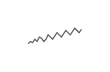
\begin{tikzpicture}[x=0.08em, y=0.08em, line width=0.4pt]
                \draw[FooterGray] (0,3) -- (1,4) -- (2,3.5) -- (3,5) -- (4,4) -- (5,6) -- (6,5.5) -- (7,4) -- (8,5) -- (9,7) -- (10,6) -- (11,5) -- (12,6.5) -- (13,8) -- (14,7) -- (15,6) -- (16,7.5) -- (17,9) -- (18,8) -- (19,7) -- (20,8.5) -- (21,10) -- (22,9) -- (23,8) -- (24,9.5);
            \end{tikzpicture}%
        }%
        \hskip0.5cm%
    }%
    \vskip6pt%
}

%=============================================================================
% PACKAGES
%=============================================================================
\usepackage[utf8]{inputenc}
\DeclareUnicodeCharacter{03B1}{\ensuremath{\alpha}}
\usepackage[T1]{fontenc}
\usepackage{amsmath, amssymb, amsthm}
\usepackage{mathtools}
\usepackage{bm}
\usepackage{tikz}
\usetikzlibrary{arrows.meta, positioning, shapes, calc, decorations.pathreplacing, shadings}
\usepackage{booktabs}
\usepackage{multirow}
\usepackage{array}
\usepackage{graphicx}
\usepackage{animate}
\usepackage{hyperref}
\usepackage{colortbl}
\usepackage{listings}
\lstset{language=Python, basicstyle=\ttfamily\scriptsize, keywordstyle=\color{MainBlue}\bfseries,
  commentstyle=\color{Forest}, stringstyle=\color{Crimson}, breaklines=true,
  frame=none, backgroundcolor=\color{VeryLightGray}, xleftmargin=2mm}
\hypersetup{colorlinks=true, linkcolor=MainBlue, urlcolor=MainBlue}
\graphicspath{{../../logos/}{../../charts/}{../../photos/}}
\usepackage{xcolor}
\hfuzz=2pt  % Suppress tiny overfull warnings (<2pt)
\vfuzz=2pt  % Suppress tiny vertical overfull warnings (<2pt)
% \mathrm in the sans-serif family of the slides (beamer resets \mathrm to the serif family at \begin{document};
% this hook runs after beamer's, so WN, Var, RMSE, ... in formulas match the surrounding text)
% Bold vectors and matrices in the same sans-serif family: \mathbf{A} in sans bold (beamer's own \mathbf came out in
% medium weight), and the bold upright Greek capitals of \boldsymbol / \bm (\bSigma, \bPhi, \boldsymbol{\Theta}) in
% cmss bold: bm.sty fixes its "boldoperators" font when it is loaded (serif cmbx), before beamer switches the
% operators to cmss, so it is reset here.
\AtBeginDocument{%
  \SetMathAlphabet{\mathrm}{normal}{\encodingdefault}{\sfdefault}{\mddefault}{n}%
  \SetMathAlphabet{\mathrm}{bold}{\encodingdefault}{\sfdefault}{bx}{n}%
  \SetMathAlphabet{\mathbf}{normal}{\encodingdefault}{\sfdefault}{bx}{n}%
  \SetMathAlphabet{\mathbf}{bold}{\encodingdefault}{\sfdefault}{bx}{n}%
  \SetSymbolFont{boldoperators}{normal}{OT1}{cmss}{bx}{n}%
  \SetSymbolFont{boldoperators}{bold}{OT1}{cmss}{bx}{n}}

%=============================================================================
% QUANTLET COMMANDS
%   \quantlet{<displayed name>}{<url>}       (generic, compatible with the older TSA decks)
%   \tsaquantlet{Ch_05}{TSA_ch5_garch}       -> https://github.com/danpele/Time-Series-Analysis/tree/main/Quantlets/Ch_05/TSA_ch5_garch
%   \qlurl{<folder>} is defined per chapter by the generator (Quantlets/Ch_NN/<folder>)
%=============================================================================
\newcommand{\tsarepo}{https://github.com/danpele/Time-Series-Analysis}
\newcommand{\tsaqlbase}{https://github.com/danpele/Time-Series-Analysis/tree/main/Quantlets}
\newcommand{\quantlet}[2]{%
    \hfill\href{#2}{%
        \raisebox{-0.15em}{
\includegraphics[height=0.7em]{ql_logo.png}}%
        \textcolor{MainBlue}{\tiny\ #1}%
    }%
}
\newcommand{\tsaquantlet}[2]{\quantlet{\detokenize{#2}}{\tsaqlbase/#1/#2}}

%=============================================================================
% NOTEBOOKS (Google Colab)
%   \colaburl{notebooks/EN/chapter5_seminar_notebook.ipynb} -> the Colab link of a file in the TSA repo
%   \nb: the chapter notebook (each seminar deck redefines it with \renewcommand)
%=============================================================================
\newcommand{\colaburl}[1]{https://colab.research.google.com/github/danpele/Time-Series-Analysis/blob/main/#1}
\newcommand{\nb}{https://colab.research.google.com/github/danpele/Time-Series-Analysis/tree/main/notebooks/EN}
\newcommand{\nbname}{notebooks/EN}

%=============================================================================
% SLIDE HELPERS (used by the generators; the same as in MFM)
%=============================================================================
% local font size for list bodies (the preamble forces \normalsize)
\newcommand{\itemsize}[1]{\setbeamertemplate{itemize/enumerate body begin}{#1}\setbeamertemplate{itemize/enumerate subbody begin}{#1}}
\newcommand{\intitle}[1]{{\hypersetup{urlcolor=white}#1}}   % white links inside coloured title bars
\newcommand{\imgcap}[1]{{\scriptsize #1}\\[0.5mm]}          % caption under a photo
\newcommand{\imgcredit}[2]{{\tiny\color{FooterGray}\href{#1}{#2}}}   % image credit: source URL, author/licence
\newcommand{\aiprompt}[1]{{\ttfamily\color{MainBlue}#1}}     % a prompt to an AI assistant

%=============================================================================
% SEMINARS: student version by default; the instructor wrapper *_solutions.tex sets \solutionstrue
%=============================================================================
\makeatletter\@ifundefined{ifsolutions}{\expandafter\newif\csname ifsolutions\endcsname}{}\makeatother
\newcommand{\solonly}[1]{\ifsolutions #1\fi}
\newcommand{\propsub}{\ifsolutions\else\framesubtitle{\ifdefined\tsalang Rezolvarea se discută la seminar\else Solution discussed in class\fi}\fi}

%=============================================================================
% APPENDIX AND CHAPTER LINKS (latex/appendix_links.py writes the calls; it also re-declares these
% macros before \begin{document}, so the decks compile with or without this preamble block)
%=============================================================================
\providecommand{\tsaapplink}[3]{\hypertarget{#2}{}\hyperlink{#1}{\beamergotobutton{#3}}}
\providecommand{\tsaappback}[2]{\begin{tikzpicture}[remember picture,overlay]\node[anchor=south east] at ([xshift=-3mm,yshift=7mm]current page.south east){\hyperlink{#1}{\beamerreturnbutton{#2}}};\end{tikzpicture}}
\providecommand{\tsachlink}[2]{\href{#1}{#2}}
\providecommand{\tsachlinkt}[2]{\href{#1}{\usebeamercolor[fg]{frametitle}#2}}

%=============================================================================
% QUANTINAR COMMAND: link către un curs Quantinar (subiecte avansate)
%=============================================================================
\newcommand{\quantinar}[2]{%
    \href{#2}{%
        \raisebox{-0.15em}{
\includegraphics[height=0.8em]{qr_logo.png}}%
        \textcolor{MainBlue}{\scriptsize\ #1}%
    }%
}

%=============================================================================
% CUSTOM TITLE PAGE
%=============================================================================
\defbeamertemplate*{title page}{hybrid}[1][]
{
    \vspace{0.2cm}
    % Logos row - top header (with clickable links)
    \begin{center}
        \href{https://www.ase.ro}{
\includegraphics[height=1.0cm]{ase_logo.png}}\hspace{0.3cm}%
        \href{https://theida.net}{
\includegraphics[height=1.0cm]{ida_logo.png}}\hspace{0.3cm}%
        \href{https://blockchain-research-center.com}{
\includegraphics[height=1.0cm]{brc_logo.png}}\hspace{0.3cm}%
        \href{https://www.ai4efin.ase.ro}{
\includegraphics[height=1.0cm]{ai4efin_logo.png}}\hspace{0.3cm}%
        \href{https://ipe.ro/new}{
\includegraphics[height=1.0cm]{acad_logo.png}}\hspace{0.3cm}%
        \href{https://www.digital-finance-msca.com}{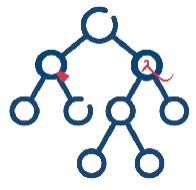
\includegraphics[height=1.0cm]{msca_logo.png}}%
    \end{center}

    \vspace{0.6cm}

    % Main title with Q logos on sides (with clickable links)
    \begin{center}
        \begin{minipage}{0.1\textwidth}
            \centering
            \href{https://quantlet.com}{
\includegraphics[height=1.1cm]{ql_logo.png}}
        \end{minipage}%
        \begin{minipage}{0.78\textwidth}
            \centering
            {\LARGE\bfseries\usebeamercolor[fg]{title}\inserttitle}

            \vspace{0.3cm}

            {\usebeamerfont{subtitle}\usebeamercolor[fg]{title}\insertsubtitle}
        \end{minipage}%
        \begin{minipage}{0.1\textwidth}
            \centering
            \href{https://quantinar.com}{
\includegraphics[height=1.1cm]{qr_logo.png}}
        \end{minipage}
    \end{center}

    \vspace{0.6cm}

    % Authors (left aligned)
    \hspace{0.5cm}{\usebeamerfont{author}\insertauthor}

    \vspace{0.3cm}

    % Institute/Affiliations (left aligned)
    \hspace{0.5cm}\begin{minipage}[t]{0.9\textwidth}
        \raggedright\small\insertinstitute
    \end{minipage}
}

%=============================================================================
% THEOREM ENVIRONMENTS
%=============================================================================
\theoremstyle{definition}
\setbeamertemplate{theorems}[numbered]
\ifdefined\tsalang
\newtheorem{defn}{Definiție}
\newtheorem{thm}{Teoremă}
\newtheorem{prop}{Propoziție}
\newtheorem{rmk}{Observație}
\else
\newtheorem{defn}{Definition}
\newtheorem{thm}{Theorem}
\newtheorem{prop}{Proposition}
\newtheorem{rmk}{Remark}
\fi

%=============================================================================
% CENTRED MINIPAGE (no extra vertical space)
%=============================================================================
\newenvironment{cminipage}[1]{%
    \par\noindent\hfill\begin{minipage}{#1}\ignorespaces
}{%
    \end{minipage}\hfill\null\par
}

%=============================================================================
% CUSTOM COMMANDS
%=============================================================================
\newcommand{\E}{\mathbb{E}}
\newcommand{\Var}{\text{Var}}
\newcommand{\Cov}{\text{Cov}}
\newcommand{\Corr}{\text{Corr}}
\newcommand{\R}{\mathbb{R}}
\newcommand{\N}{\mathbb{N}}
\newcommand{\Z}{\mathbb{Z}}
\newcommand{\B}{\mathbf{B}}
\newcommand{\imark}{\textcolor{MainBlue}{\textbullet}}
\newcommand{\RMSE}{\text{RMSE}}
\newcommand{\MAE}{\text{MAE}}
\newcommand{\MAPE}{\text{MAPE}}

% Boldface vector/matrix commands (VAR, VECM, state space; also used by the older TSA decks)
\newcommand{\bY}{\mathbf{Y}}
\newcommand{\bX}{\mathbf{X}}
\newcommand{\bA}{\mathbf{A}}
\newcommand{\bB}{\mathbf{B}}
\newcommand{\bepsilon}{\boldsymbol{\varepsilon}}
\newcommand{\bSigma}{\boldsymbol{\Sigma}}
\newcommand{\bPhi}{\boldsymbol{\Phi}}
\newcommand{\bGamma}{\boldsymbol{\Gamma}}
\newcommand{\bPi}{\boldsymbol{\Pi}}
\newcommand{\bc}{\mathbf{c}}
\newcommand{\balpha}{\boldsymbol{\alpha}}
\newcommand{\bbeta}{\boldsymbol{\beta}}
\newcommand{\bvarepsilon}{\boldsymbol{\varepsilon}}

% Legacy seminar marks (older TSA seminar decks)
\newcommand{\correct}{\textcolor{Forest}{\checkmark}}
\newcommand{\incorrect}{\textcolor{Crimson}{\texttimes}}


\newcommand{\qlurl}[1]{https://github.com/danpele/Time-Series-Analysis/tree/main/Quantlets/Ch_11/#1}

% Clickable citations (DOIs verified via Crossref)
\newcommand{\refHP}{\href{https://doi.org/10.1007/978-3-031-13584-2}{Huang and Petukhina (2022)}}
\newcommand{\refFPP}{\href{https://otexts.com/fpp3/}{Hyndman and Athanasopoulos (2021)}}
\newcommand{\refBommasani}{\href{https://arxiv.org/abs/2108.07258}{Bommasani et al.\ (2021)}}
\newcommand{\refVaswani}{\href{https://arxiv.org/abs/1706.03762}{Vaswani et al.\ (2017)}}
\newcommand{\refNie}{\href{https://arxiv.org/abs/2211.14730}{Nie et al.\ (2023)}}
\newcommand{\refAnsari}{\href{https://arxiv.org/abs/2403.07815}{Ansari et al.\ (2024)}}
\newcommand{\refAnsariB}{\href{https://arxiv.org/abs/2510.15821}{Ansari et al.\ (2025)}}
\newcommand{\refDas}{\href{https://arxiv.org/abs/2310.10688}{Das et al.\ (2024)}}
\newcommand{\refWoo}{\href{https://arxiv.org/abs/2402.02592}{Woo et al.\ (2024)}}
\newcommand{\refRasul}{\href{https://arxiv.org/abs/2310.08278}{Rasul et al.\ (2023)}}
\newcommand{\refGarza}{\href{https://arxiv.org/abs/2310.03589}{Garza et al.\ (2023)}}
\newcommand{\refGruver}{\href{https://arxiv.org/abs/2310.07820}{Gruver et al.\ (2023)}}
\newcommand{\refTan}{\href{https://arxiv.org/abs/2406.16964}{Tan et al.\ (2024)}}
\newcommand{\refZeng}{\href{https://doi.org/10.1609/aaai.v37i9.26317}{Zeng et al.\ (2023)}}
\newcommand{\refAksu}{\href{https://arxiv.org/abs/2410.10393}{Aksu et al.\ (2024)}}
\newcommand{\refMonash}{\href{https://arxiv.org/abs/2105.06643}{Godahewa et al.\ (2021)}}
\newcommand{\refSalinas}{\href{https://doi.org/10.1016/j.ijforecast.2019.07.001}{Salinas et al.\ (2020)}}
\newcommand{\refMH}{\href{https://doi.org/10.1016/S0169-2070(00)00057-1}{Makridakis and Hibon (2000)}}
\newcommand{\refMSA}{\href{https://doi.org/10.1016/j.ijforecast.2019.04.014}{Makridakis et al.\ (2020)}}
\newcommand{\refHK}{\href{https://doi.org/10.1016/j.ijforecast.2006.03.001}{Hyndman and Koehler (2006)}}
\newcommand{\refMW}{\href{https://doi.org/10.1287/mnsc.22.10.1087}{Matheson and Winkler (1976)}}
\newcommand{\refGR}{\href{https://doi.org/10.1198/016214506000001437}{Gneiting and Raftery (2007)}}
\newcommand{\refHew}{\href{https://doi.org/10.1007/s10618-022-00894-5}{Hewamalage et al.\ (2023)}}
\newcommand{\refDM}{\href{https://doi.org/10.1080/07350015.1995.10524599}{Diebold and Mariano (1995)}}

\title[Time Series Analysis]{Time Series Analysis}
\subtitle{Chapter 11: Foundation models for time series}
\author[D.T. Pele]{Daniel Traian PELE}
\institute{Bucharest University of Economic Studies\\
IDA Institute Digital Assets\\
Blockchain Research Center\\
AI4EFin Artificial Intelligence for Energy Finance\\
Romanian Academy, Institute for Economic Forecasting\\
MSCA Digital Finance}
\date{}

%=============================================================================
\providecommand{\tsaapplink}[3]{\hypertarget{#2}{}\hyperlink{#1}{\beamergotobutton{#3}}}  % APPLINKS-MACROS
\providecommand{\tsaappback}[2]{\begin{tikzpicture}[remember picture,overlay]\node[anchor=south east] at ([xshift=-3mm,yshift=7mm]current page.south east){\hyperlink{#1}{\beamerreturnbutton{#2}}};\end{tikzpicture}}  % APPLINKS-MACROS
\providecommand{\tsachlink}[2]{\href{#1}{#2}}  % APPLINKS-MACROS
\providecommand{\tsachlinkt}[2]{\href{#1}{\usebeamercolor[fg]{frametitle}#2}}  % APPLINKS-MACROS
\begin{document}
%=============================================================================

{
\setbeamertemplate{headline}{}
\setbeamertemplate{footline}{}
\begin{frame}[noframenumbering]
    \titlepage
\end{frame}
}
% BEGIN-ACRONYMS (generat de latex/acronyms.py; nu editati manual)
\begin{frame}{Acronyms used in this material (1/2)}
\setbeamertemplate{itemize/enumerate body begin}{\footnotesize}
\begin{columns}[T]
\begin{column}{0.49\textwidth}
\begin{itemize}\setlength{\itemsep}{0pt}
    \item \textbf{AI}: Artificial Intelligence
    \item \textbf{AIC}: Akaike Information Criterion
    \item \textbf{API}: Application Programming Interface
    \item \textbf{AR}: AutoRegressive (model)
    \item \textbf{ARIMA}: AutoRegressive Integrated Moving Average (model)
    \item \textbf{BNR}: Banca Națională a României (the National Bank of Romania)
    \item \textbf{BY-NC}: Attribution–NonCommercial (Creative Commons licence terms)
\end{itemize}
\end{column}
\begin{column}{0.49\textwidth}
\begin{itemize}\setlength{\itemsep}{0pt}
    \item \textbf{CDF}: Cumulative Distribution Function
    \item \textbf{CPU}: Central Processing Unit
    \item \textbf{CRPS}: Continuous Ranked Probability Score
    \item \textbf{ENTSO-E}: European Network of Transmission System Operators for Electricity
    \item \textbf{ETS}: Error, Trend, Seasonality (exponential smoothing state space models)
    \item \textbf{FRED}: Federal Reserve Economic Data
    \item \textbf{GARCH}: Generalised AutoRegressive Conditional Heteroskedasticity
\end{itemize}
\end{column}
\end{columns}
\end{frame}
\begin{frame}{Acronyms used in this material (2/2)}
\setbeamertemplate{itemize/enumerate body begin}{\footnotesize}
\begin{columns}[T]
\begin{column}{0.49\textwidth}
\begin{itemize}\setlength{\itemsep}{0pt}
    \item \textbf{GDP}: Gross Domestic Product
    \item \textbf{GIFT}: General Time Series Forecasting Model Evaluation (GIFT-Eval benchmark)
    \item \textbf{GPT}: Generative Pre-trained Transformer
    \item \textbf{GPU}: Graphics Processing Unit
    \item \textbf{HICP}: Harmonised Index of Consumer Prices
    \item \textbf{INS}: Institutul Național de Statistică — the National Institute of Statistics (Romania)
    \item \textbf{LLM}: Large Language Model
\end{itemize}
\end{column}
\begin{column}{0.49\textwidth}
\begin{itemize}\setlength{\itemsep}{0pt}
    \item \textbf{LOTSA}: Large-scale Open Time Series Archive (Moirai pretraining corpus)
    \item \textbf{MAE}: Mean Absolute Error
    \item \textbf{MASE}: Mean Absolute Scaled Error
    \item \textbf{RMSE}: Root Mean Squared Error
    \item \textbf{US}: United States
    \item \textbf{VAR}: Vector AutoRegression
    \item \textbf{WQL}: Weighted Quantile Loss
\end{itemize}
\end{column}
\end{columns}
\end{frame}
% END-ACRONYMS

\begin{frame}{Today's question and route}
\itemsize{\small}
\begin{itemize}
    \item \textbf{Question}: can one large model, pretrained on many series, forecast a series it has never seen as well as a model built for that series?
    \begin{itemize}
        \item until now (\tsachlink{https://danpele.github.io/Time-Series-Analysis/EN/Courses/chapter0_introduction.pdf}{Chapters 0}--\tsachlink{https://danpele.github.io/Time-Series-Analysis/EN/Courses/chapter10_state_space_kalman_markov_switching.pdf}{10}): one model per series, estimated on that series (ETS, ARIMA, GARCH, VAR)
        \item \tsachlink{https://danpele.github.io/Time-Series-Analysis/EN/Courses/chapter9_machine_learning_time_series.pdf}{Chapter 9}: global machine-learning models, trained on the series of one data set
    \end{itemize}
    \item \textbf{Route} of the chapter (self-study)
    \begin{itemize}
        \item the idea of a foundation model; Transformers and attention in brief
        \item from numbers to tokens: scaling, quantisation, patching; the main model families
        \item probabilistic forecasts and their scores; an honest test on Romanian and US series
        \item leakage and contamination; when these models help and when they do not
    \end{itemize}
\end{itemize}
\end{frame}

\begin{frame}{Learning outcomes}
\itemsize{\small}
\begin{itemize}
    \item Define a foundation model, zero-shot forecasting and fine-tuning
    \item Explain how a series becomes the input of a Transformer: mean scaling, quantisation, patching
    \item Describe Chronos, TimesFM, Moirai, Lag-Llama and TimeGPT and say how they differ
    \item Score a quantile forecast with the pinball loss, the CRPS, MASE and the coverage of an interval
    \item Run an open model on a CPU, compare it fairly with seasonal naive, ETS and ARIMA and recognise contamination
\end{itemize}
\end{frame}

\begin{frame}{Prerequisites for Today}
\itemsize{\footnotesize}
\begin{itemize}
    \item Forecasting benchmarks and their evaluation (\tsachlink{https://danpele.github.io/Time-Series-Analysis/EN/Courses/chapter0_introduction.pdf}{Chapters 0} and \tsachlink{https://danpele.github.io/Time-Series-Analysis/EN/Courses/chapter4_seasonality_forecasting.pdf}{4})
    \begin{itemize}
        \item seasonal naive $\hat y_{T+h} = y_{T+h-m}$: the forecast repeats the value of the same season one cycle earlier
        \item $T$: the last observed period; $h$: the horizon; $m$: the season length (12 for monthly data, 168 for hourly data with a weekly cycle); the hat marks a forecast
        \item ETS; time-series cross-validation with a rolling origin; MAE, RMSE, MASE; the Diebold--Mariano test
    \end{itemize}
    \item ARIMA and seasonal ARIMA (\tsachlink{https://danpele.github.io/Time-Series-Analysis/EN/Courses/chapter3_unit_roots_arima_models.pdf}{Chapters 3} and \tsachlink{https://danpele.github.io/Time-Series-Analysis/EN/Courses/chapter4_seasonality_forecasting.pdf}{4}); machine learning basics (\tsachlink{https://danpele.github.io/Time-Series-Analysis/EN/Courses/chapter9_machine_learning_time_series.pdf}{Chapter 9})
    \begin{itemize}
        \item training, validation and test samples; a neural network as a flexible function with many parameters
        \item global models: one model trained on many series
    \end{itemize}
    \item Quantiles: $q_\tau$ is the value below which the variable falls with probability $\tau$
    \begin{itemize}
        \item $\tau \in (0, 1)$: the level; $q_{0.5}$ is the median, $q_{0.1}$ and $q_{0.9}$ bound a central 80\% interval
    \end{itemize}
\end{itemize}
\end{frame}


%=============================================================================
\section{The foundation-model idea}
%=============================================================================

\begin{frame}{Three ways to forecast many series}
\itemsize{\small}
\begin{itemize}
    \item \textbf{Local} models
    \begin{itemize}
        \item one model per series, estimated on that series only
        \item ETS, ARIMA: few parameters, interpretable; 10\,000 series mean 10\,000 estimations
    \end{itemize}
    \item \textbf{Global} models (\tsachlink{https://danpele.github.io/Time-Series-Analysis/EN/Courses/chapter9_machine_learning_time_series.pdf}{Chapter 9})
    \begin{itemize}
        \item one model trained on all the series of a data set
        \item example: DeepAR (\refSalinas), a recurrent network trained on all products of a retailer
    \end{itemize}
    \item \textbf{Foundation} models
    \begin{itemize}
        \item one model pretrained once on a very broad corpus of series from many domains
        \item then used on new series and new data sets, without re-estimation
        \item the term comes from \refBommasani: models trained on broad data at scale, adaptable to many tasks
    \end{itemize}
\end{itemize}
\end{frame}

\begin{frame}{Zero-shot, fine-tuning, in-context}
\itemsize{\small}
\begin{itemize}
    \item \textbf{Context}
    \begin{itemize}
        \item the recent history $y_{T-C+1}, \dots, y_T$ passed to the model at forecast time ($C$ = context length)
    \end{itemize}
    \item \textbf{Zero-shot} forecasting
    \begin{itemize}
        \item the pretrained weights stay fixed
        \item only the context of the new series is used
        \item no parameter is estimated on the target series: forecasting takes a fraction of a second
    \end{itemize}
    \item \textbf{Fine-tuning}
    \begin{itemize}
        \item further training of the pretrained weights on the target data
        \item can help on unusual series; needs a validation sample and more computation
    \end{itemize}
    \item The output is usually a set of \textbf{quantiles} $\hat q_{0.1}, \dots, \hat q_{0.9}$ for each future step, not a single number
\end{itemize}
\end{frame}

\begin{frame}{Pretraining at scale}
\itemsize{\small}
\begin{columns}[T]
\begin{column}{0.42\textwidth}
\centering
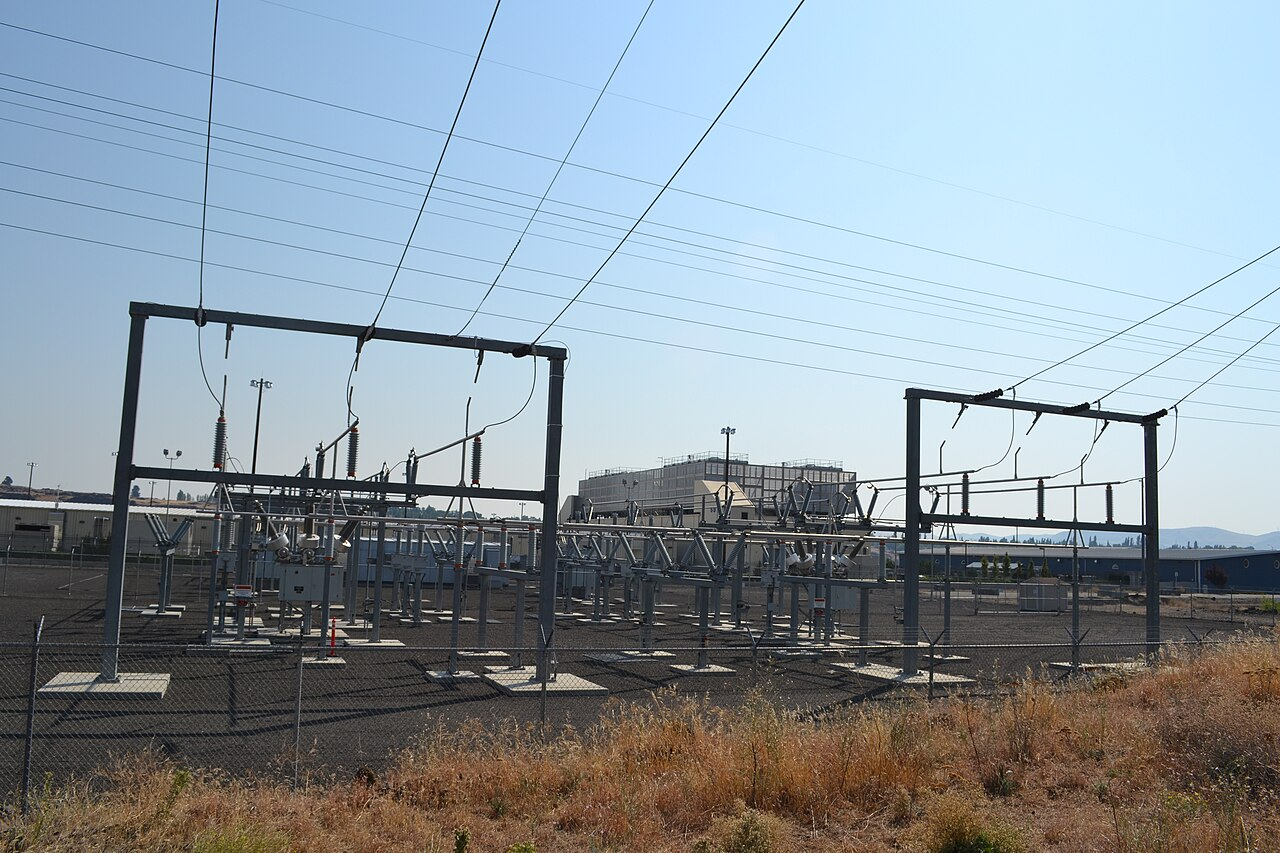
\includegraphics[height=0.46\textheight]{ch11_google_dalles_2011.jpg}\\[1mm]
\imgcap{A Google data centre, The Dalles, Oregon}
\imgcredit{https://commons.wikimedia.org/wiki/File:Google_Data_Center,_The_Dalles.jpg}{Photo: Visitor7 (2011); CC BY-SA 3.0; Wikimedia Commons}
\end{column}
\begin{column}{0.56\textwidth}
\begin{itemize}
    \item Pretraining corpora mix public series from many domains
    \begin{itemize}
        \item energy, transport, retail, weather, web traffic, finance and economics
        \item plus synthetic series: random mixtures of real series and series drawn from Gaussian processes (Chronos)
    \end{itemize}
    \item Scale: TimesFM was pretrained on about $10^{11}$ time points (\refDas)
    \item Pretraining is done once, by the developer, on many graphics processors (GPU)
    \begin{itemize}
        \item the user only runs the model: the small versions run on an ordinary CPU
    \end{itemize}
\end{itemize}
\end{column}
\end{columns}
\end{frame}

\begin{frame}{Recap: The foundation-model idea}
\itemsize{\small}
\begin{itemize}
    \item Local, global and foundation models differ in what the model is trained on
    \item Zero-shot: fixed weights, only the context of the new series
    \item The output is a set of quantiles: a probabilistic forecast
\end{itemize}
\end{frame}


%=============================================================================
\section{Transformers in brief}
%=============================================================================

\begin{frame}{The Transformer (Vaswani et al., 2017)}
\itemsize{\small}
\begin{columns}[T]
\begin{column}{0.34\textwidth}
\centering
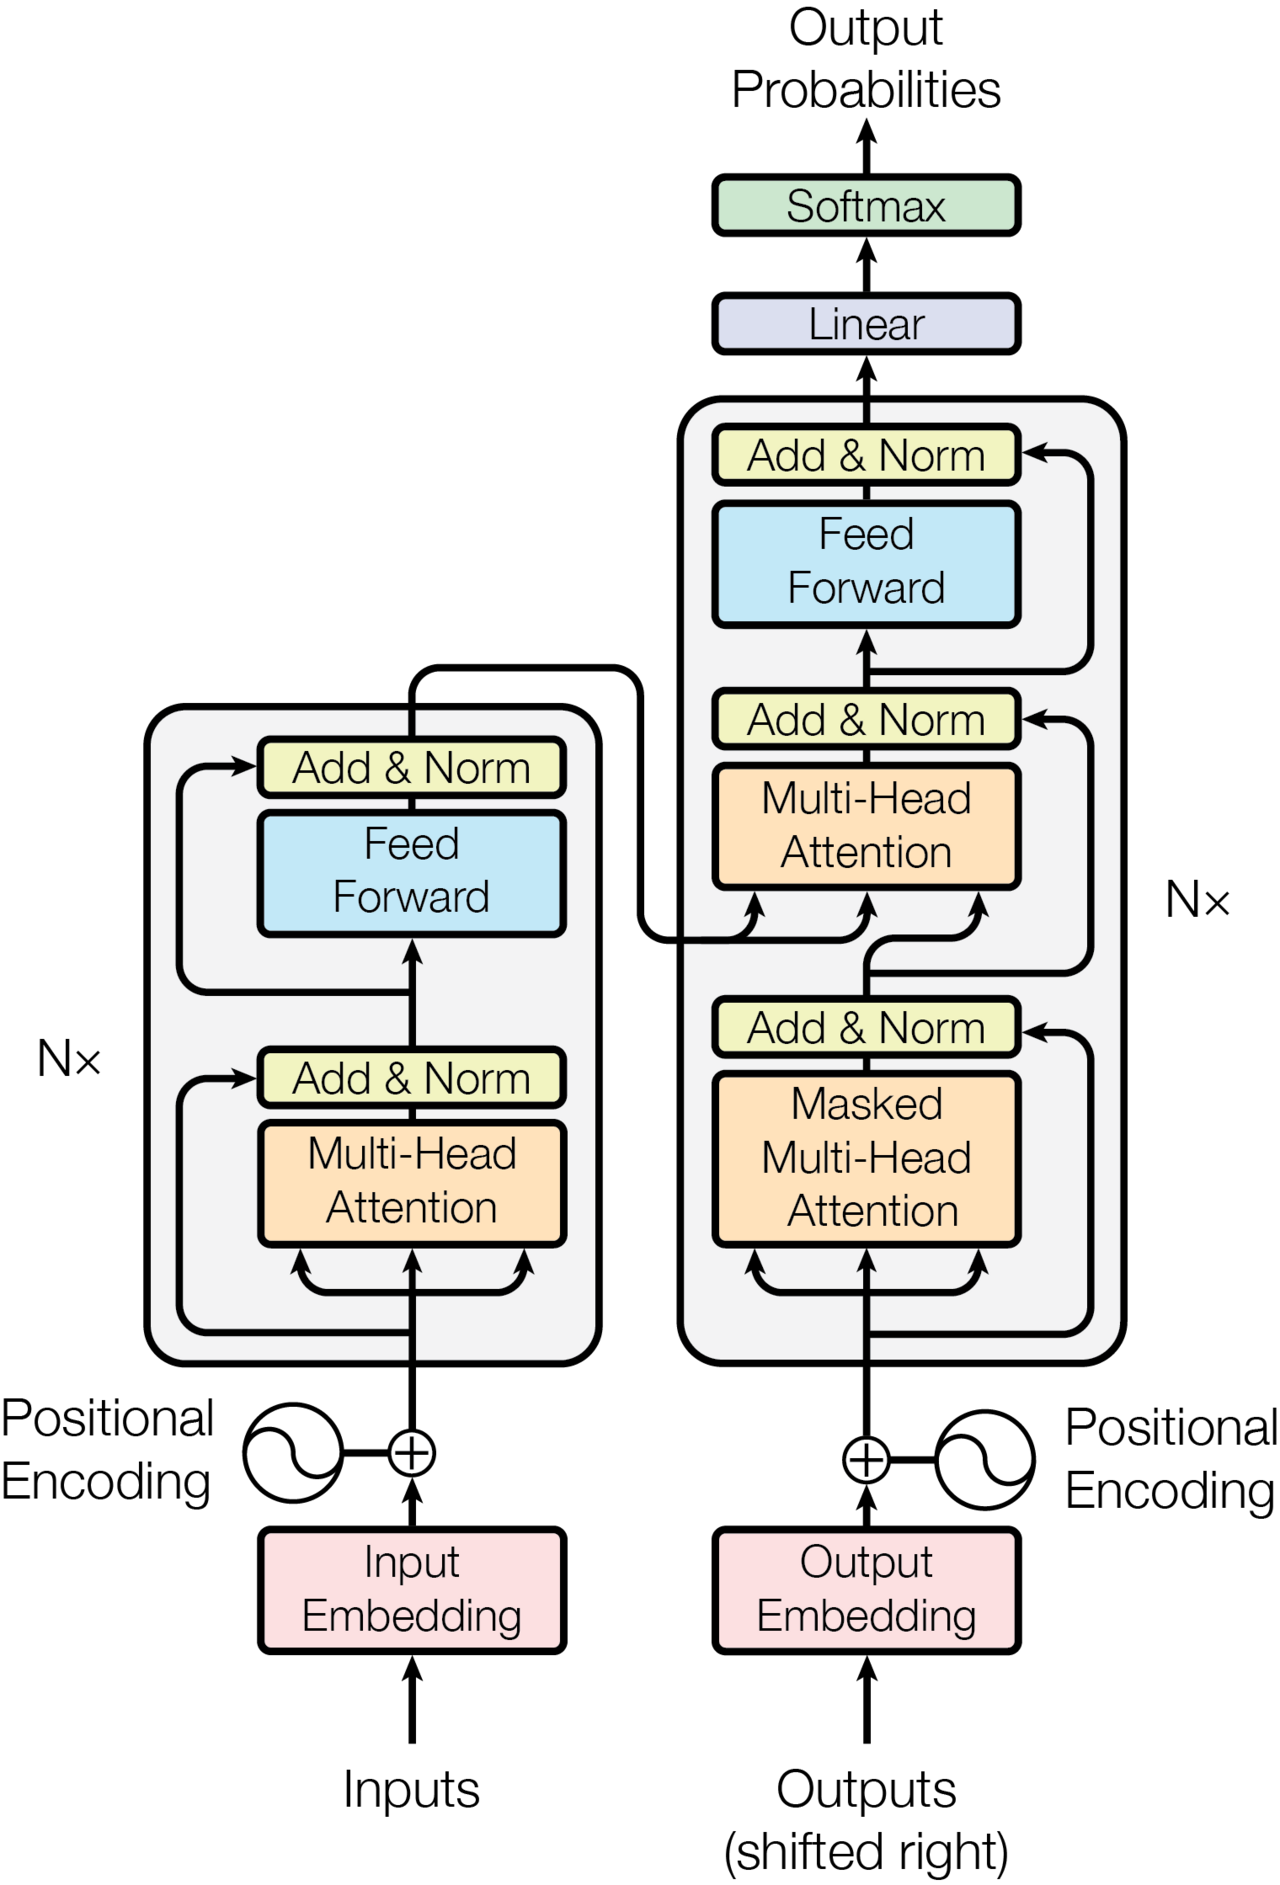
\includegraphics[height=0.62\textheight]{ch11_attention_figure_2017.png}\\[1mm]
\imgcap{The original diagram: encoder (left), decoder (right)}
\imgcredit{https://commons.wikimedia.org/wiki/File:Attention_Is_All_You_Need_-_Encoder-decoder_Architecture.png}{Figure: Vaswani et al.\ (2017), Google; CC BY-SA 4.0; Wikimedia Commons}
\end{column}
\begin{column}{0.64\textwidth}
\begin{itemize}
    \item \refVaswani: a network for sequences built on \textbf{attention}, without recurrence
    \begin{itemize}
        \item designed for translation; behind every large language model (LLM)
    \end{itemize}
    \item Input: a sequence of \textbf{tokens}, each turned into a vector (an embedding)
    \item \textbf{Encoder--decoder} architecture
    \begin{itemize}
        \item the \textbf{encoder} reads the whole input
        \item the \textbf{decoder} produces the output step by step
        \item \textbf{decoder-only} models (GPT, TimesFM, Lag-Llama) forecast the next token from all previous ones
    \end{itemize}
    \item Position information is added to each vector, since attention ignores order
\end{itemize}
\end{column}
\end{columns}
\end{frame}

\begin{frame}{Self-attention (1/2): the formula}
\itemsize{\footnotesize}
\begin{itemize}
    \item Each input vector $x_i$ produces three vectors, by three linear maps learnt in training
    \begin{itemize}
        \item a query $q_i = W_Q x_i$ (what position $i$ looks for), a key $k_i = W_K x_i$ (what position $i$ offers), a value $v_i = W_V x_i$ (what position $i$ passes on)
        \item $W_Q$, $W_K$, $W_V$: weight matrices learnt in training, the same for every position
    \end{itemize}
    \item The output at position $i$ is a weighted average of the values of all positions
    \begin{itemize}
        \item $\displaystyle \text{out}_i = \sum_j w_{ij} v_j, \qquad w_{ij} = \frac{\exp(q_i^\top k_j/\sqrt{d})}{\sum_l \exp(q_i^\top k_l/\sqrt{d})}$
    \end{itemize}
    \item Notation
    \begin{itemize}
        \item $j, l$: indices that run over all input positions; $w_{ij}$: the weight that position $i$ gives to position $j$
        \item $q_i^\top k_j$: the scalar product of query and key, large when the two vectors point in the same direction (similarity score)
        \item $d$: the length of the key vectors; dividing by $\sqrt{d}$ keeps the scores of moderate size
        \item the exponential makes every weight positive and the denominator makes the weights of position $i$ sum to 1
    \end{itemize}
\end{itemize}
\end{frame}

\begin{frame}{Self-attention (2/2): matrix form and intuition}
\itemsize{\small}
\begin{itemize}
    \item Matrix form of the same computation: $\text{softmax}(QK^\top/\sqrt{d})\,V$
    \begin{itemize}
        \item $Q$, $K$, $V$: matrices whose rows are the vectors $q_i$, $k_i$, $v_i$; $QK^\top$ holds all the scores $q_i^\top k_j$
        \item softmax: applied row by row, it turns the scores into the weights $w_{ij}$ of the previous slide
    \end{itemize}
    \item Intuition for series: today's step can look back at the same hour last week and give it a large weight
    \begin{itemize}
        \item the weights are learnt from data, not fixed in advance as the lags of an AR($p$)
    \end{itemize}
    \item Cost: $n$ inputs need $n^2$ comparisons
    \begin{itemize}
        \item a context of 2048 values gives about 4 million comparisons in each attention layer
    \end{itemize}
\end{itemize}
\end{frame}

\begin{frame}{Worked example: attention weights}
\itemsize{\small}
\begin{itemize}
    \item One query and three keys; scores $q^\top k_j/\sqrt{d}$ = 2, 1, 0; values $v_j$ = 10, 20, 30
    \item Step 1: exponentiate: $e^2$, $e^1$, $e^0$
    \item Step 2: divide by the sum: weights 0.67, 0.24, 0.09 (they sum to 1)
    \item Step 3: output $= \sum_j w_j v_j$ = 14.2
    \begin{itemize}
        \item the highest score gets most of the weight, but every value contributes
    \end{itemize}
    \item A foundation model stacks many such layers, each with several attention heads
\end{itemize}
\end{frame}

\begin{frame}{Recap: Transformers}
\itemsize{\small}
\begin{itemize}
    \item Attention: each step is a learnt weighted average of all steps
    \item Encoder--decoder (Chronos) and decoder-only (TimesFM, Lag-Llama) designs
    \item The cost grows with the square of the number of inputs
\end{itemize}
\end{frame}


%=============================================================================
\section{From numbers to tokens}
%=============================================================================

\begin{frame}{The problem: a language model reads words, a series has numbers}
\itemsize{\small}
\begin{itemize}
    \item Series differ in units and levels: load in GW, an index around 100, an exchange rate around 5
    \begin{itemize}
        \item one model for all of them needs a common scale
    \end{itemize}
    \item Three solutions used in practice
    \begin{itemize}
        \item \textbf{scaling + quantisation}: each value becomes one token from a fixed vocabulary (Chronos)
        \item \textbf{patching}: groups of consecutive values become one input vector (TimesFM, Moirai, Chronos-Bolt)
        \item \textbf{digits as text}: a general LLM reads the numbers as strings (\refGruver)
    \end{itemize}
    \item In all cases the forecasts are transformed back to the original units
\end{itemize}
\end{frame}

\begin{frame}{Mean scaling and quantisation (Chronos) (1/2)}
\itemsize{\footnotesize}
\begin{itemize}
    \item \textbf{Mean scaling}
    \begin{itemize}
        \item each value of the context is divided by the mean absolute value of the context
        \item $\tilde x_t = x_t / s, \qquad s = \frac{1}{C}\sum_{t=1}^{C} |x_t|$
        \item $x_t$: the $t$-th value of the context, $t = 1, \dots, C$; $C$: the context length; $s$: the scale; $\tilde x_t$: the scaled value
        \item the scaled context has values of order one, whatever the units
    \end{itemize}
    \item \textbf{Quantisation}
    \begin{itemize}
        \item each scaled value is replaced by the number of a bin
        \item $[-15, 15]$ is divided into 4093 equal bins of width 0.0073; the token of $\tilde x_t$ is the number of the nearest bin centre
        \item plus special tokens (padding, end of sequence)
    \end{itemize}
\end{itemize}
\end{frame}

\begin{frame}{Mean scaling and quantisation (Chronos) (2/2)}
\itemsize{\small}
\begin{itemize}
    \item Training: a language model (T5) learns to predict the next token
    \begin{itemize}
        \item loss: the cross-entropy $-\log \hat p(z_{t+1})$, where $z_{t+1}$ is the true next token and $\hat p(z_{t+1})$ the probability the model gave it
        \item it is 0 when that probability is 1 and grows as the probability falls
    \end{itemize}
    \item Forecast in three steps
    \begin{itemize}
        \item sample many token paths from the model
        \item map each token back to its bin centre and multiply by $s$
        \item read the quantiles of the sampled values at each future step
    \end{itemize}
    \item Limit: scaled values outside $[-15, 15]$ cannot be produced
\end{itemize}
\end{frame}

\begin{frame}{Worked example: scaling and tokens}
\itemsize{\small}
\begin{itemize}
    \item Context: the Romanian unemployment rate (\%, seasonally adjusted, Eurostat), March 2026 to August 2026
    \begin{itemize}
        \item $x$ = 6.5, 6.8, 6.7, 6.8, 6.4, 6.4
    \end{itemize}
    \item Step 1: scale $s$ = mean of $|x_t|$ = 6.60
    \item Step 2: scaled values $x_t/s$ = 0.985, 1.030, 1.015, 1.030, 0.970, 0.970
    \item Step 3: nearest bin centres (0 to 4092): tokens 2180, 2187, 2184, 2187, 2178, 2178
    \begin{itemize}
        \item equal values give equal tokens; a change of 0.1 points moves the token by several bins
    \end{itemize}
    \item The model never sees the level 6.6\%: only the shape relative to the scale
\end{itemize}
\end{frame}

\begin{frame}{Scaling and quantisation on real data (1/2)}
\itemsize{\small}
\centering
\makebox[\textwidth][c]{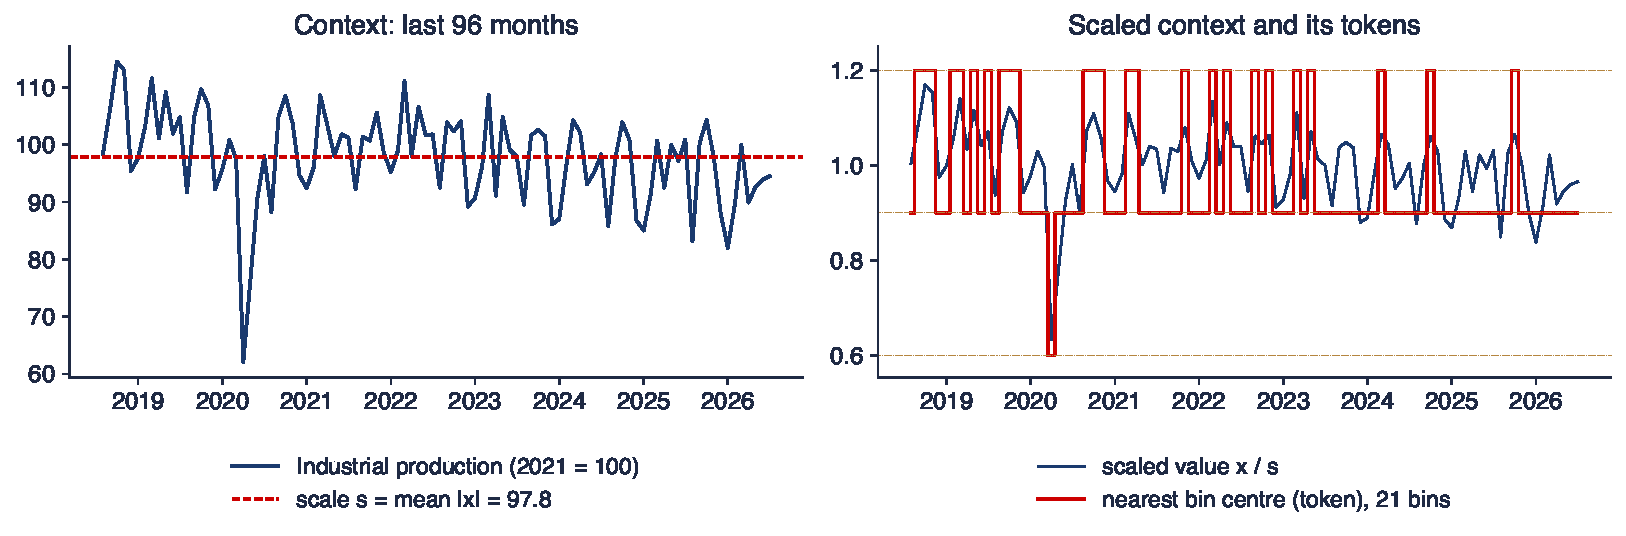
\includegraphics[width=0.96\paperwidth,height=0.88\textheight,keepaspectratio]{tsa_ch11_tokens.pdf}}
\end{frame}

\begin{frame}{Scaling and quantisation on real data (2/2)}
\itemsize{\small}
\begin{itemize}
    \item Romanian industrial production (Eurostat, 2021 = 100), the last 96 months; scale $s$ = 97.8
    \item Right: the scaled context and its tokens on a coarse grid of 21 bins (Chronos uses 4093)
\end{itemize}
\quantlet{TSA\_ch11\_tokens\_scores}{\qlurl{TSA_ch11_tokens_scores}}
\end{frame}

\begin{frame}{Interpreting the tokens}
\itemsize{\small}
\begin{itemize}
    \item After scaling, all values lie between 0.63 and 1.17: a few per cent of the range $[-15, 15]$
    \item On the coarse grid the 96 months use only 3 tokens: the April 2020 fall (the lockdown) is one separate token
    \item With 4093 bins the grid is fine enough to keep the seasonal shape
    \item One extreme value inflates $s$ and shrinks all the other scaled values: outliers in the context matter
\end{itemize}
\end{frame}

\begin{frame}{Patching}
\itemsize{\small}
\begin{itemize}
    \item \textbf{Patch}
    \begin{itemize}
        \item a block of $P$ consecutive values, mapped to one input vector by a small network
        \item PatchTST (\refNie): ``a time series is worth 64 words''
    \end{itemize}
    \item Two gains
    \begin{itemize}
        \item fewer inputs: 2048 values with $P = 16$ give 128 patches, so attention needs $128^2$ instead of $2048^2$ comparisons
        \item each input carries a local shape (a slope, a peak), not a single noisy number
    \end{itemize}
    \item Used by TimesFM (input patches of 32), Moirai (patch size by frequency), Chronos-Bolt and Chronos-2 (16)
    \begin{itemize}
        \item the output can also be a whole patch of future values at once, which is faster than token by token
    \end{itemize}
\end{itemize}
\end{frame}

\begin{frame}{Patching the Romanian electricity load}
\itemsize{\footnotesize}
\begin{center}
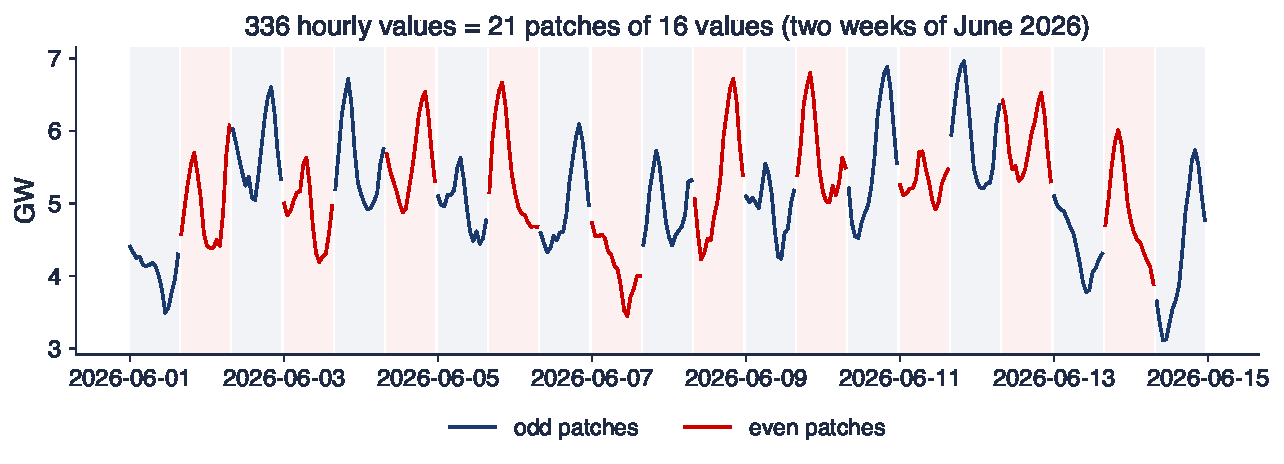
\includegraphics[width=0.97\textwidth,height=0.62\textheight,keepaspectratio]{tsa_ch11_patching.pdf}
\end{center}
\vspace{-0.25cm}
\begin{itemize}
    \item 336 hourly values (two weeks of June 2026, ENTSO-E) cut into 21 patches of 16 values
\end{itemize}
\quantlet{TSA\_ch11\_tokens\_scores}{\qlurl{TSA_ch11_tokens_scores}}
\end{frame}

\begin{frame}{Interpreting patching}
\itemsize{\small}
\begin{itemize}
    \item A day has 24 hours, so a patch of 16 covers two thirds of a day: patches do not align with the daily cycle
    \item Attention links patches: the morning rise of Monday can be matched with that of the previous Monday
    \item A weekly cycle (168 hours) is visible only if the context covers at least one week: 11 patches
\end{itemize}
\end{frame}

\begin{frame}{Recap: From numbers to tokens}
\itemsize{\small}
\begin{itemize}
    \item Mean scaling removes units; quantisation turns values into tokens (Chronos)
    \item Patching groups values: shorter sequences, local shapes
    \item The forecast is transformed back to the original units
\end{itemize}
\end{frame}


%=============================================================================
\section{The main model families}
%=============================================================================

\begin{frame}{Chronos, Chronos-Bolt and Chronos-2 (Amazon)}
\itemsize{\footnotesize}
\begin{columns}[T]
\begin{column}{0.32\textwidth}
\centering
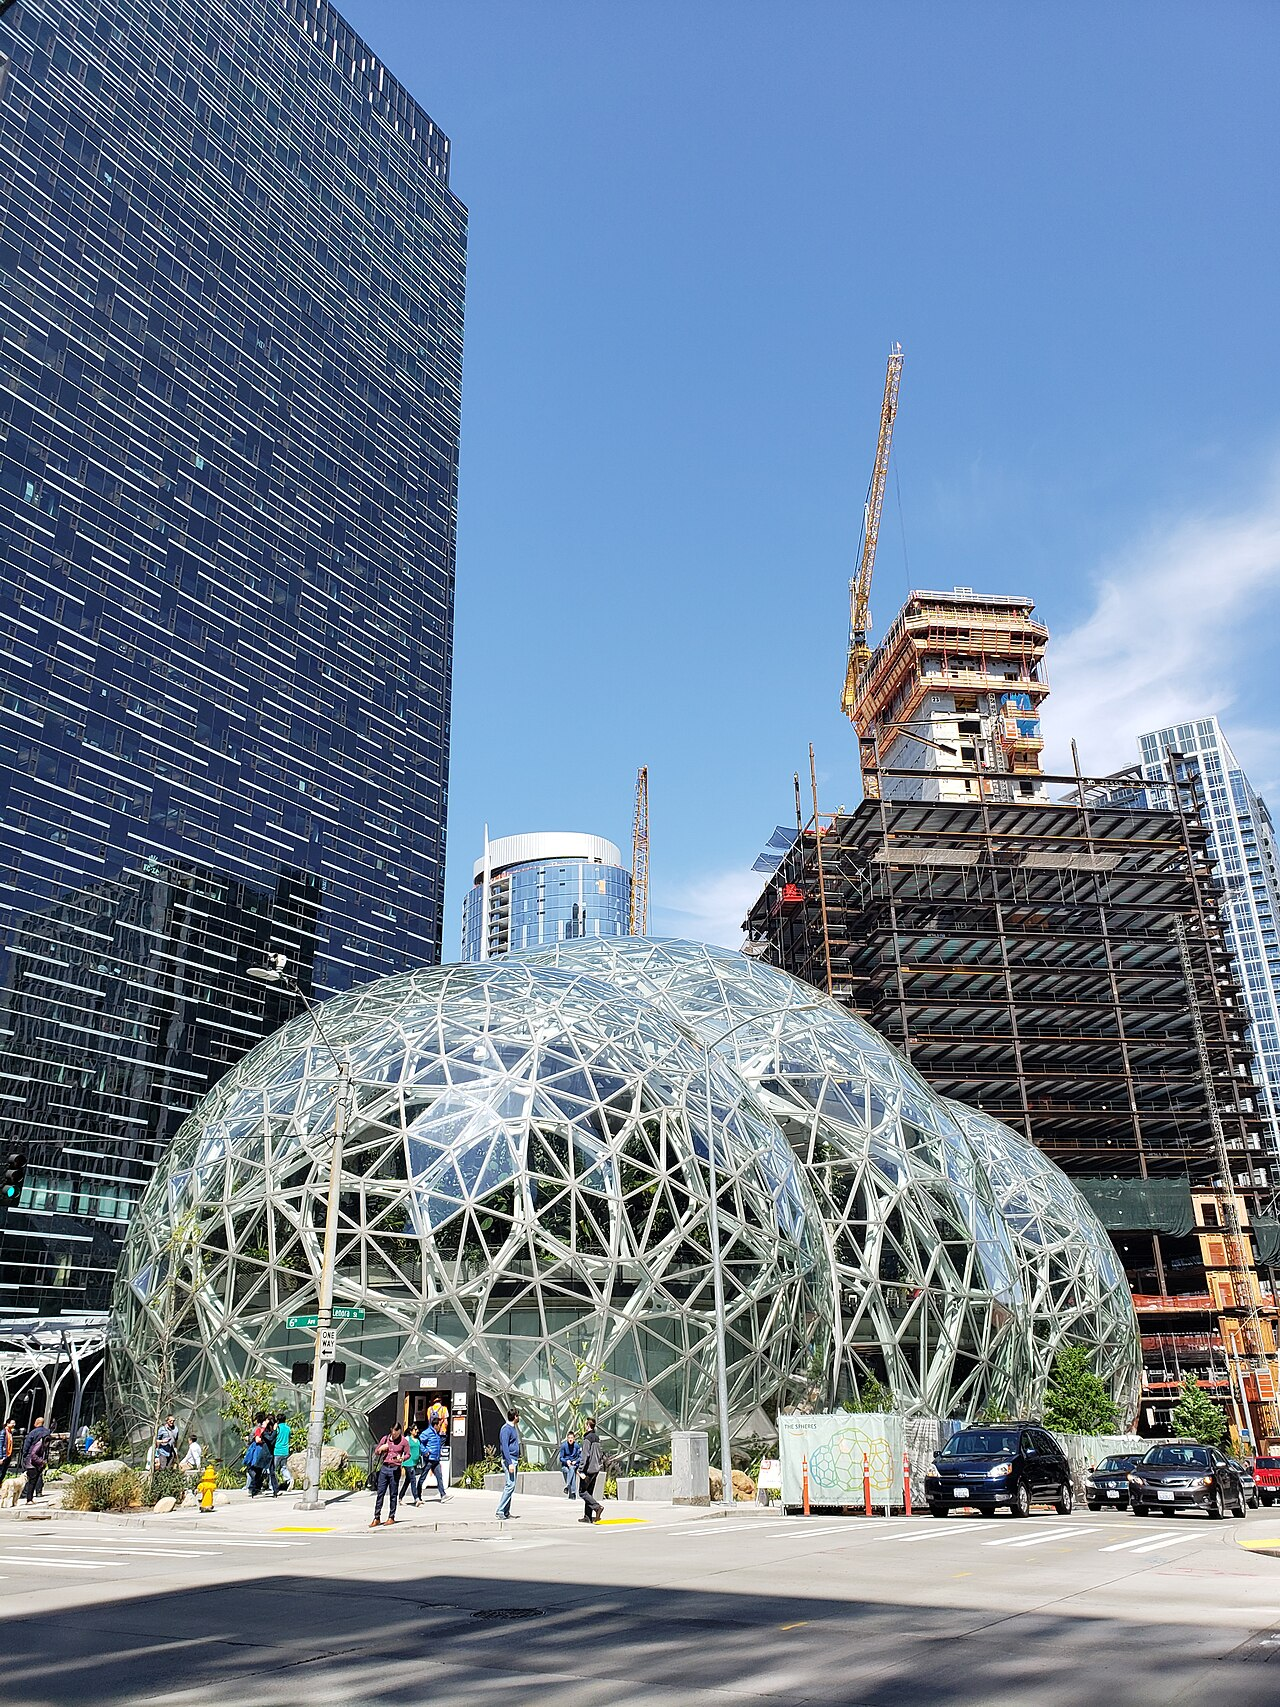
\includegraphics[height=0.62\textheight]{ch11_amazon_spheres_2018.jpg}\\[1mm]
\imgcap{The Amazon Spheres, Seattle}
\imgcredit{https://commons.wikimedia.org/wiki/File:Amazon_Spheres_2018.jpg}{Photo: Andy Li (2018); CC0; Wikimedia Commons}
\end{column}
\begin{column}{0.66\textwidth}
\begin{itemize}
    \item \textbf{Chronos} (\refAnsari)
    \begin{itemize}
        \item T5 encoder--decoder on scaled and quantised values
        \item samples token paths
    \end{itemize}
    \item \textbf{Chronos-Bolt} (November 2024)
    \begin{itemize}
        \item patches of 16 values and a direct output of the quantiles 0.1, \dots, 0.9
        \item sizes used here: tiny 9 and small 48 million parameters; context up to 2048 values
    \end{itemize}
    \item \textbf{Chronos-2} (\refAnsariB, October 2025)
    \begin{itemize}
        \item 119 million parameters, 21 quantile levels, covariates and groups of related series
    \end{itemize}
    \item Open weights (Apache-2.0 licence); Python package \texttt{chronos-forecasting}; all run on a CPU
\end{itemize}
\end{column}
\end{columns}
\end{frame}

\begin{frame}{TimesFM (Google) and Lag-Llama}
\itemsize{\footnotesize}
\begin{itemize}
    \item \textbf{TimesFM} (\refDas)
    \begin{itemize}
        \item decoder-only Transformer, input patches of 32, output patches of 128 values
        \item pretrained on real series (Google Trends, Wikipedia page views) and synthetic ones; about 200 million parameters
        \item open weights (Apache-2.0); later versions add quantile outputs
    \end{itemize}
    \item \textbf{Lag-Llama} (\refRasul)
    \begin{itemize}
        \item decoder-only, built on the Llama architecture of language models
        \item inputs: lagged values chosen by frequency (for example 7 days, 12 months, 24 hours) plus calendar features
        \item output: the parameters of a Student-$t$ distribution for the next step; sampling gives paths
        \item small and open (Apache-2.0); meant to be fine-tuned
    \end{itemize}
\end{itemize}
\end{frame}

\begin{frame}{Moirai (Salesforce) and TimeGPT}
\itemsize{\footnotesize}
\begin{columns}[T]
\begin{column}{0.3\textwidth}
\centering
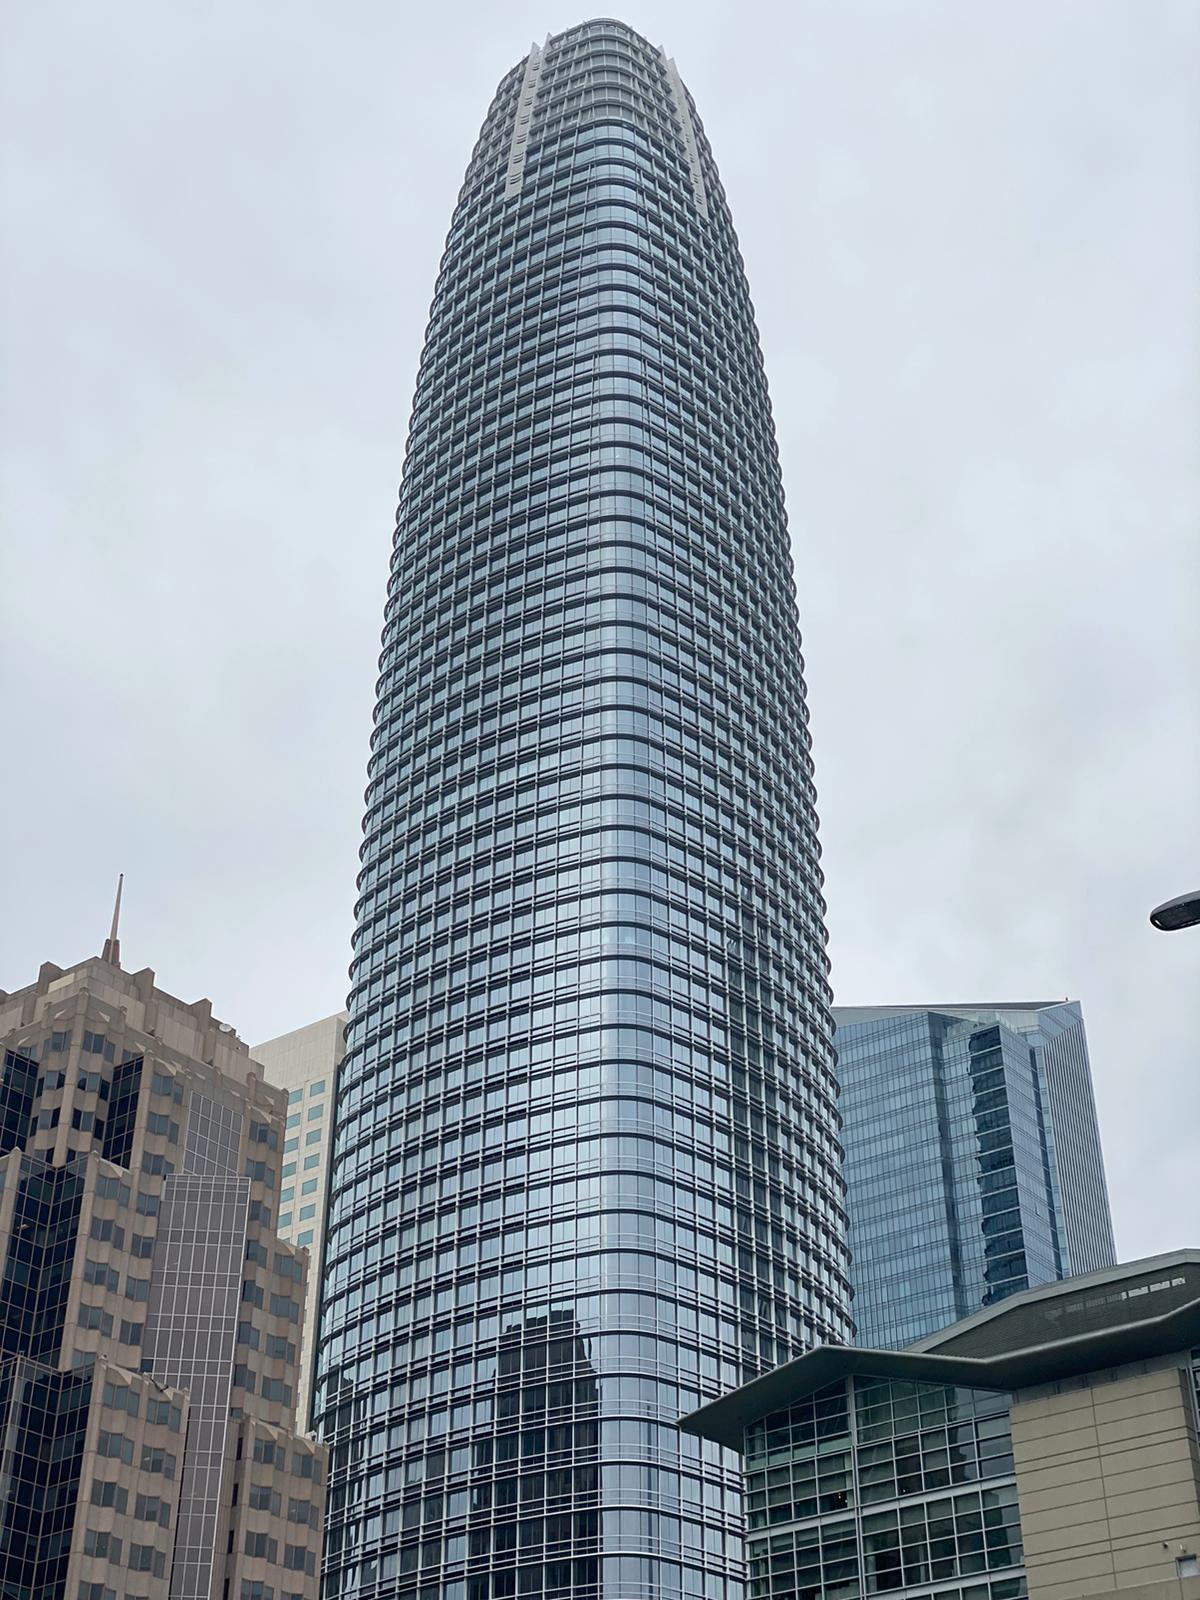
\includegraphics[height=0.62\textheight]{ch11_salesforce_tower_2020.jpg}\\[1mm]
\imgcap{Salesforce Tower, San Francisco}
\imgcredit{https://commons.wikimedia.org/wiki/File:Salesforce_Tower_2020.jpg}{Photo: Saggittarius A (2020); CC BY-SA 4.0; Wikimedia Commons}
\end{column}
\begin{column}{0.68\textwidth}
\begin{itemize}
    \item \textbf{Moirai} (\refWoo)
    \begin{itemize}
        \item ``universal'' forecaster
        \item any number of variables in one sequence; patch size chosen by frequency
        \item output: a mixture of distributions; corpus LOTSA, about 27 billion observations
        \item open weights under a non-commercial licence (CC BY-NC 4.0)
    \end{itemize}
    \item \textbf{TimeGPT} (\refGarza)
    \begin{itemize}
        \item closed model, available only through a paid API
        \item the weights and the training data cannot be inspected; the version can change; the data leave your computer
        \item not used in this course: the results could not be reproduced
    \end{itemize}
\end{itemize}
\end{column}
\end{columns}
\end{frame}

\begin{frame}{The families side by side}
\itemsize{\footnotesize}
\begin{center}
\scriptsize
\begin{tabular}{lllll}
\toprule
\textbf{Model} & \textbf{Architecture} & \textbf{Input} & \textbf{Output} & \textbf{Access} \\
\midrule
Chronos (2024) & encoder--decoder (T5) & tokens (bins) & sampled paths & Apache-2.0 \\
Chronos-Bolt (2024) & encoder--decoder & patches of 16 & 9 quantiles & Apache-2.0 \\
Chronos-2 (2025) & encoder & patches + covariates & 21 quantiles & Apache-2.0 \\
TimesFM (2024) & decoder & patches of 32 & patches of 128 & Apache-2.0 \\
Moirai (2024) & encoder & patches, any variables & mixture & CC BY-NC 4.0 \\
Lag-Llama (2023) & decoder (Llama) & lagged values & Student-$t$ & Apache-2.0 \\
TimeGPT (2023) & not disclosed & -- & points, intervals & paid API \\
\bottomrule
\end{tabular}
\end{center}
\begin{itemize}
    \item A further line of work feeds the digits to general LLMs (\refGruver); \refTan{} show that the language-model part adds cost but no accuracy
\end{itemize}
\end{frame}

\begin{frame}{Recap: The model families}
\itemsize{\small}
\begin{itemize}
    \item Chronos: tokens; Chronos-Bolt and Chronos-2: patches and direct quantiles
    \item TimesFM and Lag-Llama: decoder-only; Moirai: any number of variables
    \item Open weights make results reproducible; a paid API does not
\end{itemize}
\end{frame}


%=============================================================================
\section{Probabilistic forecasts and their scores}
%=============================================================================

\begin{frame}{Quantile forecasts}
\itemsize{\footnotesize}
\begin{itemize}
    \item A \textbf{probabilistic forecast} gives the distribution of $y_{T+h}$ given the data up to $T$
    \begin{itemize}
        \item foundation models report it through quantiles $\hat q_\tau$ at levels $\tau = 0.1, \dots, 0.9$
    \end{itemize}
    \item Point forecast: the median $\hat q_{0.5}$
    \item Central 80\% interval: $[\hat q_{0.1}, \hat q_{0.9}]$; a \textbf{fan chart} draws several such bands
    \item Two qualities to check
    \begin{itemize}
        \item \textbf{calibration}: the 80\% interval contains about 80\% of the outcomes
        \item \textbf{sharpness}: among calibrated forecasts, narrower is better (\refGR)
    \end{itemize}
    \item For ETS and ARIMA we use Normal quantiles $\hat q_\tau = \hat y_{T+h} + z_\tau \hat\sigma_h$
    \begin{itemize}
        \item $z_\tau$: the $\tau$ quantile of the standard Normal distribution ($z_{0.9} = 1.28$); $\hat\sigma_h$: the estimated standard deviation of the $h$-step forecast error
    \end{itemize}
\end{itemize}
\end{frame}

\begin{frame}{The pinball loss}
\itemsize{\small}
\begin{itemize}
    \item The \textbf{pinball} (quantile) loss scores one forecast quantile $\hat q_\tau$ against the outcome $y$
    \begin{itemize}
        \item $L_\tau(y, \hat q_\tau) = \tau\,(y - \hat q_\tau)$ if $y \ge \hat q_\tau$, and $(1 - \tau)(\hat q_\tau - y)$ otherwise
    \end{itemize}
    \item Notation
    \begin{itemize}
        \item $\tau$: the quantile level; $\hat q_\tau$: the forecast quantile; $y$: the value observed later
    \end{itemize}
    \item Reading
    \begin{itemize}
        \item the loss is 0 when $\hat q_\tau = y$ and grows linearly with the distance between them
        \item an outcome above the quantile is weighted by $\tau$, one below by $1 - \tau$
        \item its expected value is smallest at the true quantile: reporting the true quantile is the best strategy
    \end{itemize}
\end{itemize}
\end{frame}

\begin{frame}{The CRPS}
\itemsize{\footnotesize}
\begin{itemize}
    \item The \textbf{CRPS} (continuous ranked probability score, \refMW) scores a whole forecast distribution against the outcome $y$
    \begin{itemize}
        \item $\text{CRPS}(F, y) = \int (F(z) - \mathbf{1}\{z \ge y\})^2\,dz = 2\int_0^1 L_\tau(y, F^{-1}(\tau))\,d\tau$
    \end{itemize}
    \item Notation
    \begin{itemize}
        \item $F$: the forecast cumulative distribution function (CDF); $z$: the integration variable, running over all possible values
        \item $\mathbf{1}\{z \ge y\}$: the indicator, 1 if $z \ge y$ and 0 otherwise (the CDF of a forecast that puts all mass on $y$)
        \item $F^{-1}(\tau)$: the $\tau$ quantile of $F$; the second form is the pinball loss averaged over all levels
    \end{itemize}
    \item Reading
    \begin{itemize}
        \item $\text{CRPS} \ge 0$, in the units of $y$; 0 only for a forecast that puts all its mass on the outcome; smaller is better
        \item for a point forecast it equals $|y - \hat y|$: the CRPS generalises the MAE
    \end{itemize}
\end{itemize}
\end{frame}

\begin{frame}{The weighted quantile loss (WQL)}
\itemsize{\small}
\begin{itemize}
    \item \textbf{WQL} (weighted quantile loss)
    \begin{itemize}
        \item the CRPS approximated with the 9 levels 0.1, \dots, 0.9 and divided by the size of the series
        \item $\text{WQL} = \frac{1}{9}\sum_{\tau}\frac{2\sum_t L_\tau(y_t, \hat q_{\tau,t})}{\sum_t |y_t|}$
    \end{itemize}
    \item Notation
    \begin{itemize}
        \item $\tau$: runs over the 9 levels; $t$: runs over all forecast steps of all origins
        \item $\hat q_{\tau,t}$: the forecast $\tau$ quantile for step $t$; $y_t$: the outcome at step $t$
    \end{itemize}
    \item Reading
    \begin{itemize}
        \item the denominator $\sum_t |y_t|$ removes the units: series with different levels can be compared
        \item 0 for a perfect forecast; smaller is better; used by Chronos and GIFT-Eval
    \end{itemize}
\end{itemize}
\end{frame}

\begin{frame}{The pinball loss and the CRPS}
\itemsize{\footnotesize}
\begin{center}
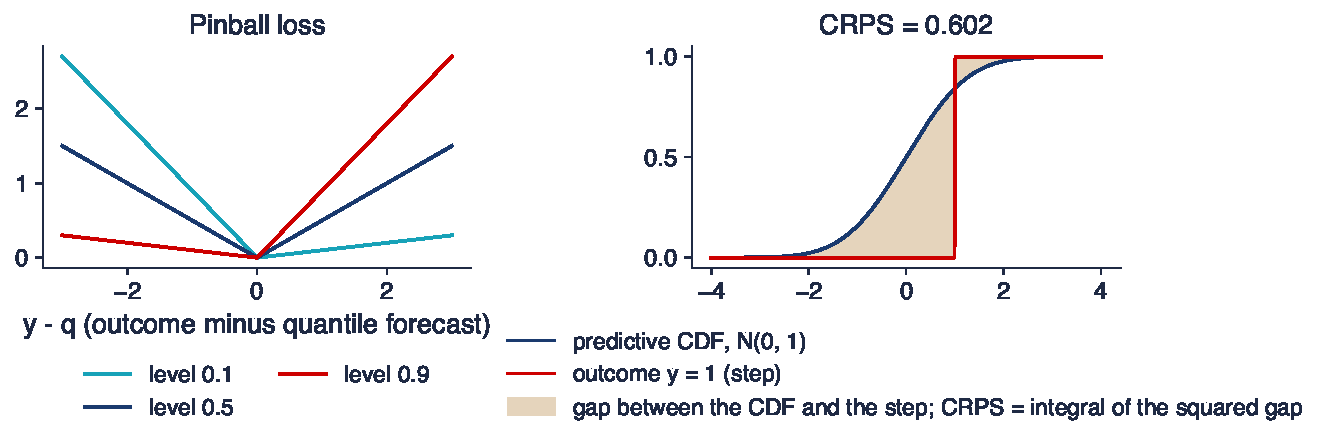
\includegraphics[width=0.97\textwidth,height=0.58\textheight,keepaspectratio]{tsa_ch11_scores.pdf}
\end{center}
\vspace{-0.25cm}
\begin{itemize}
    \item Left: $L_\tau$ against $y - \hat q$ for $\tau$ = 0.1, 0.5, 0.9. Right: the forecast N(0, 1), the outcome $y = 1$
    \item N($\mu$, $\sigma^2$): the Normal distribution with mean $\mu$ and variance $\sigma^2$
\end{itemize}
\quantlet{TSA\_ch11\_tokens\_scores}{\qlurl{TSA_ch11_tokens_scores}}
\end{frame}

\begin{frame}{Interpreting the scores}
\itemsize{\small}
\begin{itemize}
    \item At $\tau = 0.9$ an outcome above the quantile costs 9 times more than one below: the 0.9 quantile should be exceeded only 10\% of the time
    \item At $\tau = 0.5$ the loss is half the absolute error: the median is scored like a point forecast
    \item CRPS of N(0, 1): 0.234 if $y = 0$, 0.602 if $y = 1$; N(0, 4) at $y = 1$ gives 0.663: a wider band is penalised even when it covers the outcome
    \item The CRPS rewards calibration and sharpness at the same time
\end{itemize}
\end{frame}

\begin{frame}{Worked example: pinball losses}
\itemsize{\small}
\begin{itemize}
    \item Forecast of next month's unemployment rate: $\hat q_{0.1}$ = 6.5, $\hat q_{0.5}$ = 7.0, $\hat q_{0.9}$ = 7.6; outcome $y$ = 7.2
    \item $\tau = 0.1$: $y$ is above, loss $0.1 \cdot (7.2 - 6.5)$ = 0.07
    \item $\tau = 0.5$: $y$ is above, loss $0.5 \cdot (7.2 - 7.0)$ = 0.10
    \item $\tau = 0.9$: $y$ is below, loss $(1 - 0.9) \cdot (7.6 - 7.2)$ = 0.04
    \item Approximate CRPS with these three levels: $\frac{2}{3}$ (sum of losses) = 0.140 percentage points
    \begin{itemize}
        \item the outcome lies inside the 80\% interval [6.5; 7.6]: coverage indicator 1
    \end{itemize}
\end{itemize}
\end{frame}

\begin{frame}{Point accuracy: the MASE}
\itemsize{\footnotesize}
\begin{itemize}
    \item \textbf{MASE} (mean absolute scaled error, \refHK)
    \begin{itemize}
        \item the MAE of the forecast divided by the in-sample MAE of the seasonal naive
        \item $\text{MASE} = \dfrac{\frac1h\sum_{j=1}^{h}|y_{T+j} - \hat y_{T+j}|}{\frac{1}{T-m}\sum_{t=m+1}^{T}|y_t - y_{t-m}|}$
    \end{itemize}
    \item Notation
    \begin{itemize}
        \item numerator: the mean absolute error of the forecasts $\hat y_{T+j}$ over the $h$ steps after the origin $T$
        \item denominator: the mean absolute error of the seasonal naive forecast $y_{t-m}$ inside the sample $t = m+1, \dots, T$; $m$: the season length
    \end{itemize}
    \item Reading
    \begin{itemize}
        \item below 1: better than the in-sample seasonal naive; above 1: worse; free of units
        \item example: MAE 0.30, in-sample naive MAE 0.25, so MASE = 1.2
    \end{itemize}
\end{itemize}
\end{frame}

\begin{frame}{Coverage and relative scores}
\itemsize{\small}
\begin{itemize}
    \item \textbf{Coverage}
    \begin{itemize}
        \item the share of outcomes inside the 80\% interval
        \item $\text{Cov} = \frac1n\sum_{i=1}^{n} \mathbf{1}\{\hat q_{0.1}^{(i)} \le y_i \le \hat q_{0.9}^{(i)}\}$; $n$: the number of forecasts; $\hat q_{\tau}^{(i)}$: the quantile of forecast $i$; $\mathbf{1}\{\cdot\}$: 1 if the outcome is inside, 0 otherwise
        \item target 80\%; 7 of 10 inside means 70\%: intervals somewhat too narrow
    \end{itemize}
    \item \textbf{Relative scores}
    \begin{itemize}
        \item a model's MASE or WQL divided by that of the seasonal naive on the same origins
        \item below 1: the model beats the seasonal naive
        \item averaged over the $S$ series with the geometric mean $(r_1 r_2 \cdots r_S)^{1/S}$, $r_k$: the ratio for series $k$; so 2 and 0.5 cancel out
    \end{itemize}
\end{itemize}
\end{frame}

\begin{frame}{Recap: Scores}
\itemsize{\small}
\begin{itemize}
    \item Pinball loss for each quantile; CRPS for the whole distribution; WQL as its scaled approximation
    \item MASE for the median; coverage for calibration
    \item Report scores relative to the seasonal naive forecast
\end{itemize}
\end{frame}


%=============================================================================
\section{Zero-shot forecasts on real data}
%=============================================================================

\begin{frame}{Seven series for the test (1/3)}
\itemsize{\small}
\centering
\makebox[\textwidth][c]{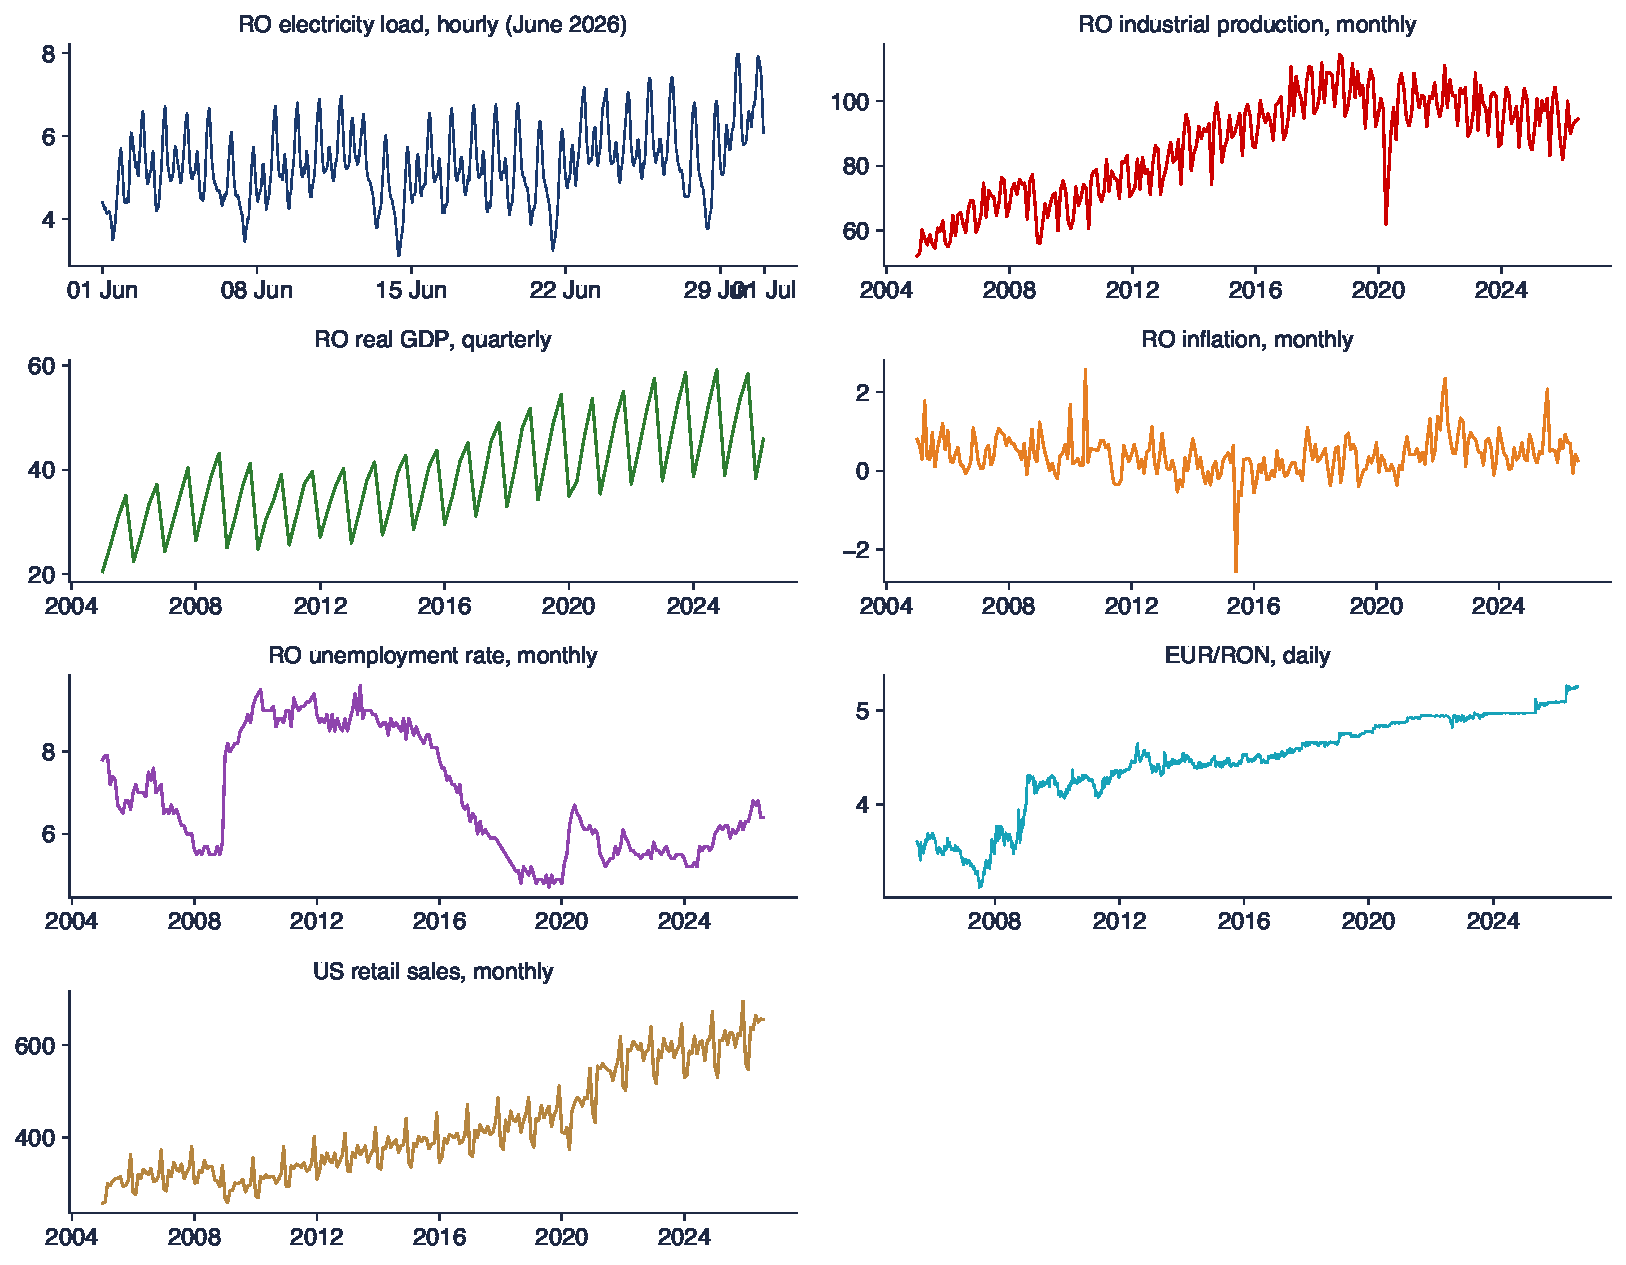
\includegraphics[trim=0 305 0 0,clip,width=0.96\paperwidth,height=0.88\textheight,keepaspectratio]{tsa_ch11_series.pdf}}
\end{frame}

\begin{frame}{Seven series for the test (2/3)}
\itemsize{\small}
\centering
\makebox[\textwidth][c]{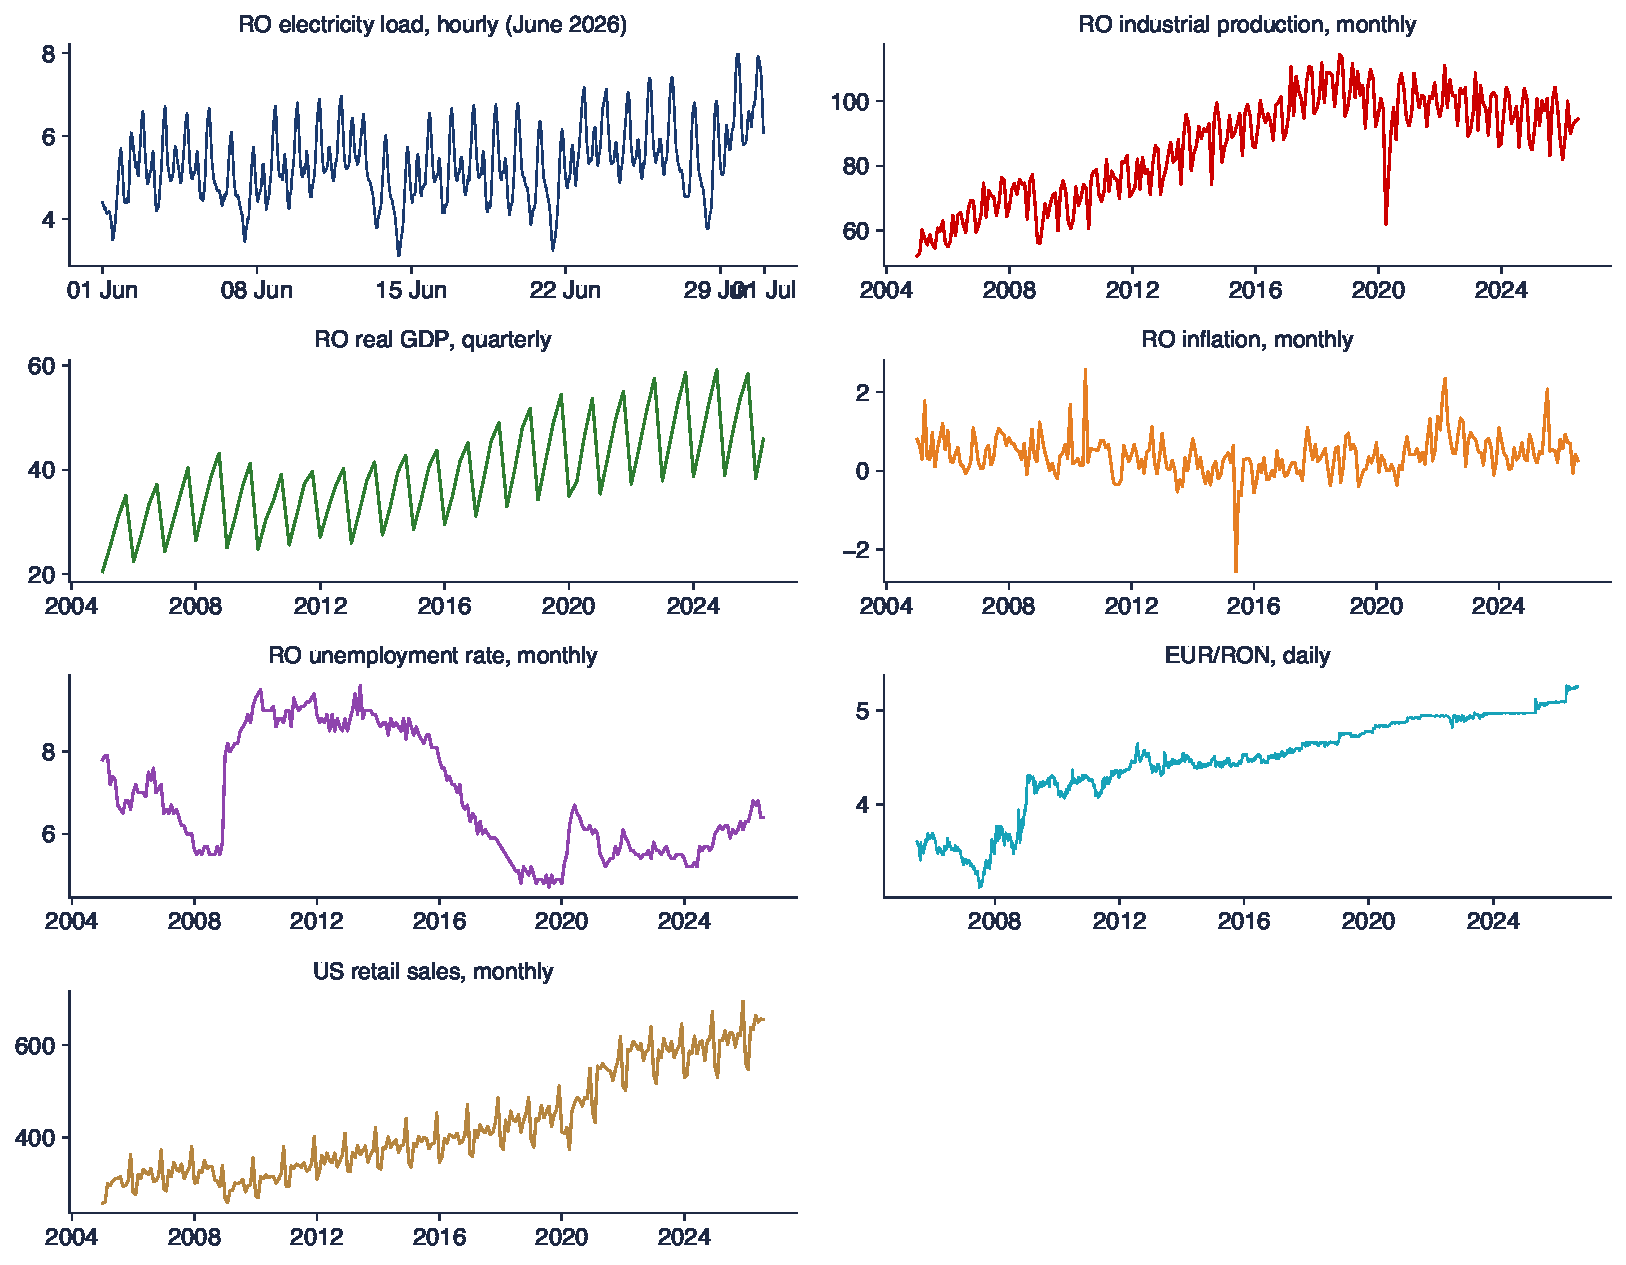
\includegraphics[trim=0 0 0 302,clip,width=0.96\paperwidth,height=0.88\textheight,keepaspectratio]{tsa_ch11_series.pdf}}
\end{frame}

\begin{frame}{Seven series for the test (3/3)}
\itemsize{\small}
\begin{itemize}
    \item Romania (ENTSO-E)
    \begin{itemize}
        \item hourly electricity load
    \end{itemize}
    \item Romania (Eurostat)
    \begin{itemize}
        \item industrial production
        \item real GDP, not seasonally adjusted
        \item HICP inflation; unemployment rate
    \end{itemize}
    \item EUR/RON (BNR reference rate)
    \item US retail sales (FRED RSXFSN)
\end{itemize}
\quantlet{TSA\_ch11\_tokens\_scores}{\qlurl{TSA_ch11_tokens_scores}}
\end{frame}

\begin{frame}{Interpreting the seven series}
\itemsize{\small}
\begin{itemize}
    \item Strong seasonality: load (daily and weekly cycles), industrial production and US retail sales (yearly), GDP (quarterly)
    \item Close to a random walk: EUR/RON and the unemployment rate; noisy and short-lived: monthly inflation
    \item Breaks: the 2020 pandemic (industrial production, GDP, retail); the 2022 inflation surge
    \item Lengths from 126 quarters (GDP) to 39\,408 hours (load): very different amounts of context
\end{itemize}
\end{frame}

\begin{frame}{Romanian electricity load, 48 hours ahead (1/2)}
\itemsize{\small}
\centering
\makebox[\textwidth][c]{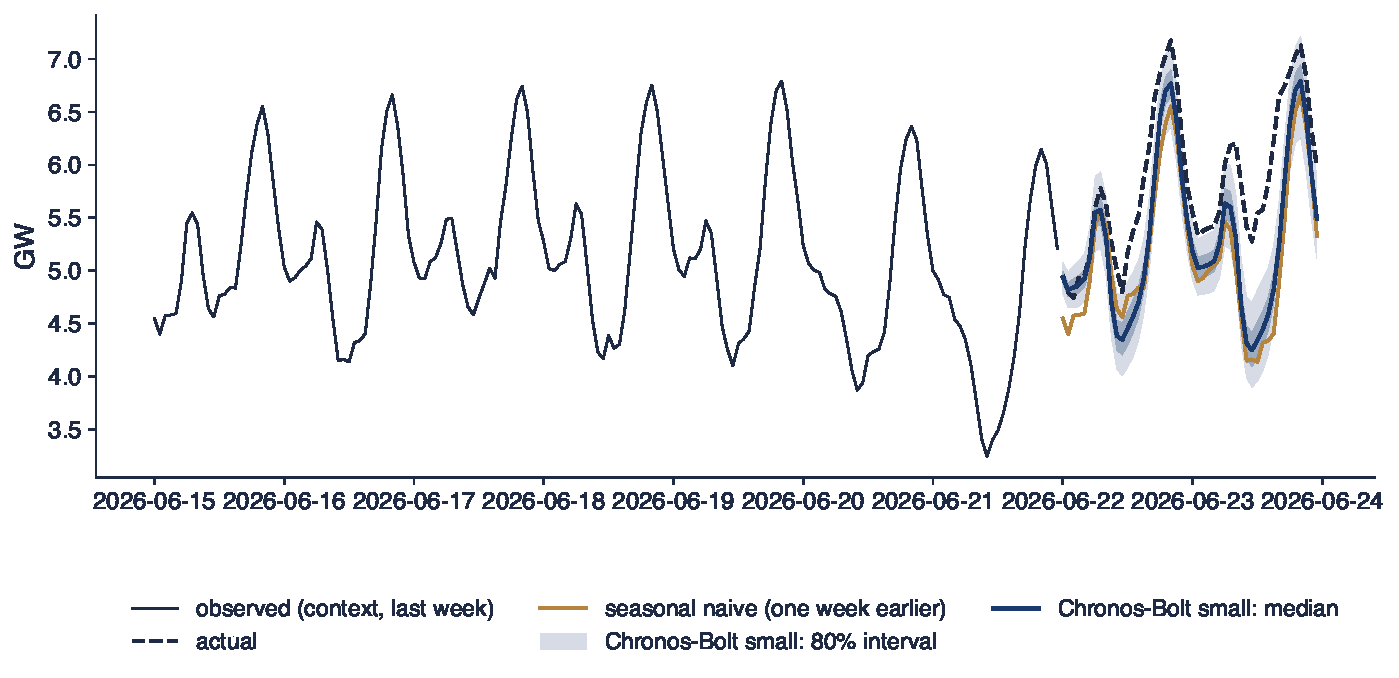
\includegraphics[width=0.96\paperwidth,height=0.88\textheight,keepaspectratio]{tsa_ch11_fan_load.pdf}}
\end{frame}

\begin{frame}{Romanian electricity load, 48 hours ahead (2/2)}
\itemsize{\small}
\begin{itemize}
    \item Chronos-Bolt small, zero-shot, context of 2048 hours (85 days); origin 22 June 2026, 00:00; bands: 50\% and 80\% central intervals
\end{itemize}
\quantlet{TSA\_ch11\_zero\_shot}{\qlurl{TSA_ch11_zero_shot}}
\end{frame}

\begin{frame}{Interpreting the load forecast}
\itemsize{\small}
\begin{itemize}
    \item The model reproduces the daily shape (night trough, evening peak) without any estimation on this series
    \item MASE: Chronos-Bolt 1.31, seasonal naive 1.61: better than repeating last week
    \item But the actual load stays above the forecast all day: only 29\% of the 48 hours fall in the 80\% band
    \item The model has no temperature or calendar input: a change in the weather that the past 85 days do not announce cannot be anticipated
    \item One origin proves little: the systematic test follows
\end{itemize}
\end{frame}

\begin{frame}{Worked example: scoring one hour}
\itemsize{\small}
\begin{itemize}
    \item Hour 24 of the load forecast (22 June 2026, 23:00): $\hat q_{0.1}$ = 5.18, $\hat q_{0.5}$ = 5.48, $\hat q_{0.9}$ = 5.78 GW; outcome 5.80 GW
    \item All three quantiles are below the outcome, so each loss is $\tau\,(y - \hat q_\tau)$
    \begin{itemize}
        \item $\tau = 0.1$: 0.062; \ $\tau = 0.5$: 0.163; \ $\tau = 0.9$: 0.025 GW
    \end{itemize}
    \item The outcome is above $\hat q_{0.9}$: coverage indicator 0 for this hour
    \item Averaged over many hours and origins, these losses give the WQL of the next section
\end{itemize}
\end{frame}

\begin{frame}{Romanian industrial production, 12 months ahead (1/2)}
\itemsize{\small}
\centering
\makebox[\textwidth][c]{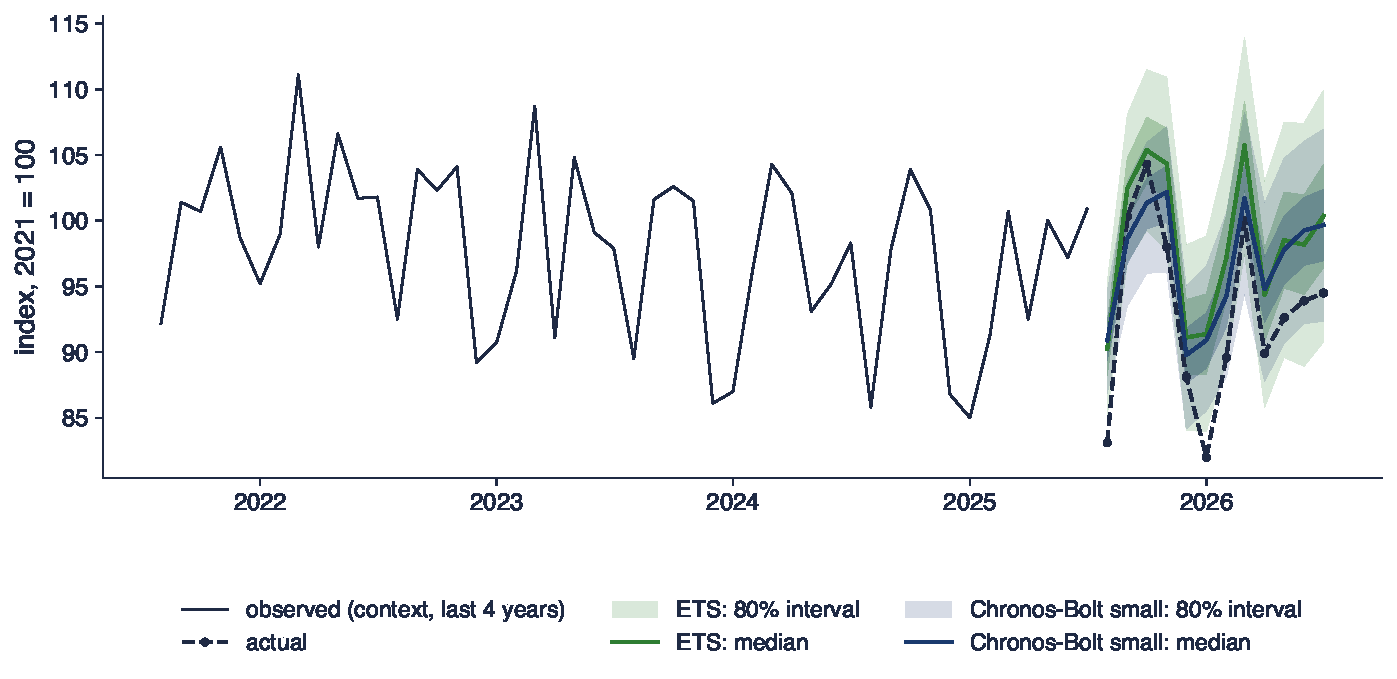
\includegraphics[width=0.96\paperwidth,height=0.88\textheight,keepaspectratio]{tsa_ch11_fan_ip.pdf}}
\end{frame}

\begin{frame}{Romanian industrial production, 12 months ahead (2/2)}
\itemsize{\small}
\begin{itemize}
    \item Origin August 2025, forecasts to July 2026; Chronos-Bolt small (zero-shot) and ETS (estimated on the series), both with 80\% bands
\end{itemize}
\quantlet{TSA\_ch11\_zero\_shot}{\qlurl{TSA_ch11_zero_shot}}
\end{frame}

\begin{frame}{Interpreting the industrial-production forecast}
\itemsize{\small}
\begin{itemize}
    \item Both models copy the seasonal pattern (the August and December dips) and keep the recent level
    \item MASE: Chronos-Bolt 1.04, ETS 1.20, seasonal naive 0.67: on this origin the simplest forecast wins
    \item The weak production of 2026 is not announced by the context; the 80\% bands cover 83\% (Chronos-Bolt) and 83\% (ETS) of the months
    \item The bands of Chronos-Bolt are narrower than those of ETS at long horizons
\end{itemize}
\end{frame}

\begin{frame}{EUR/RON, 20 days ahead (1/2)}
\itemsize{\small}
\centering
\makebox[\textwidth][c]{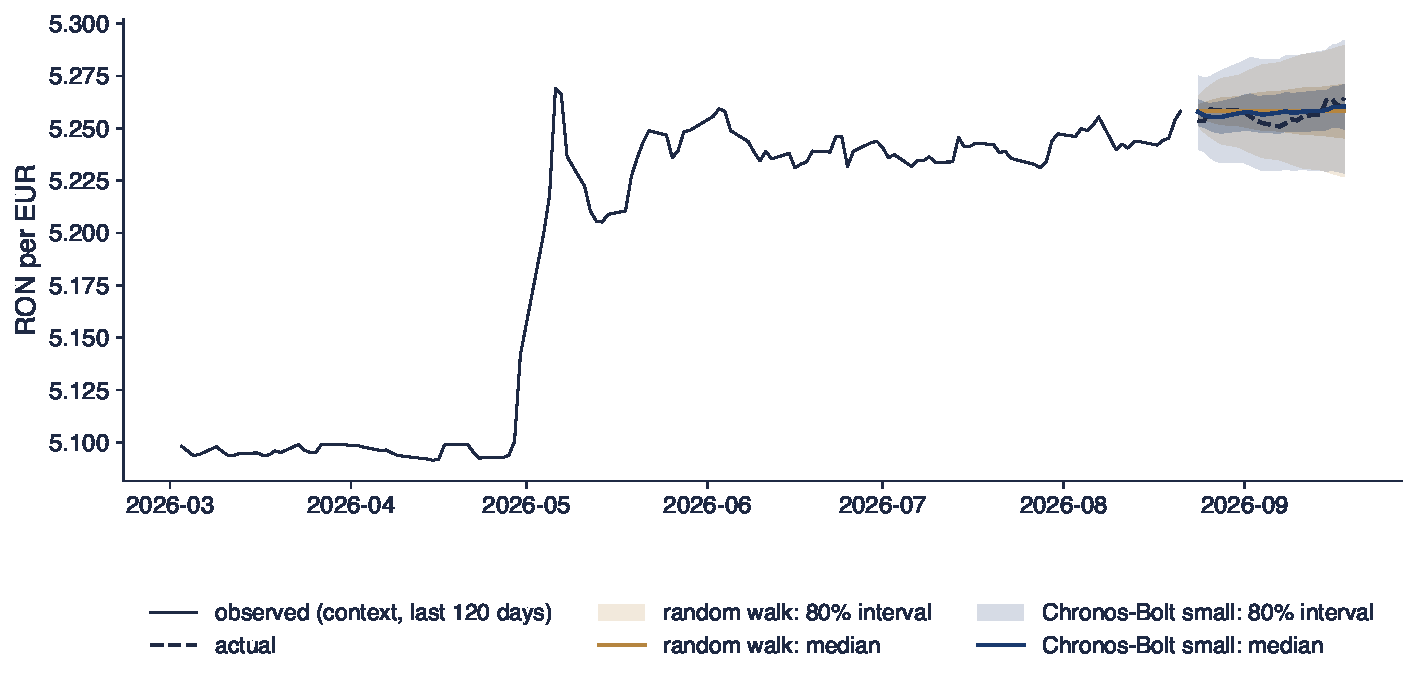
\includegraphics[width=0.96\paperwidth,height=0.88\textheight,keepaspectratio]{tsa_ch11_fan_eurron.pdf}}
\end{frame}

\begin{frame}{EUR/RON, 20 days ahead (2/2)}
\itemsize{\small}
\begin{itemize}
    \item BNR reference rate; origin 24 August 2026, last value before it 5.2581; Chronos-Bolt small against the random walk with Normal bands
\end{itemize}
\quantlet{TSA\_ch11\_zero\_shot}{\qlurl{TSA_ch11_zero_shot}}
\end{frame}

\begin{frame}{Interpreting the EUR/RON forecast}
\itemsize{\small}
\begin{itemize}
    \item The median after 20 days is 5.2604, practically the last value 5.2581: the model has learnt to behave like a random walk
    \item Width of the 80\% band at 20 days: 0.064 (Chronos-Bolt) and 0.063 (random walk): almost the same uncertainty
    \item MAE over the 20 days: 0.0032 against 0.0035: a tie in practice
    \item A model cannot extract what the past does not contain: exchange rates stay close to unpredictable (\tsachlink{https://danpele.github.io/Time-Series-Analysis/EN/Courses/chapter1_stochastic_processes_stationarity.pdf}{Chapter 1})
\end{itemize}
\end{frame}

\begin{frame}{Recap: Zero-shot forecasts}
\itemsize{\small}
\begin{itemize}
    \item Without estimation, the model copies cycles and levels from the context
    \item It cannot anticipate what the context does not show (heat, a downturn)
    \item On a random walk it returns a random walk
\end{itemize}
\end{frame}


%=============================================================================
\section{An honest evaluation}
%=============================================================================

\begin{frame}{The test protocol}
\itemsize{\footnotesize}
\begin{itemize}
    \item \textbf{Rolling origin} (\tsachlink{https://danpele.github.io/Time-Series-Analysis/EN/Courses/chapter4_seasonality_forecasting.pdf}{Chapter 4})
    \begin{itemize}
        \item at each origin every model forecasts $h$ steps from the data up to the origin only
        \item load: $h$ = 48 hours, weekly origins July 2025 to June 2026; monthly series: $h$ = 12, monthly origins from 2016; GDP: $h$ = 4, from 2012; EUR/RON: $h$ = 20 days, every 20 days from 2016
        \item 708 origins in total; context: all the past, at most 2048 observations
    \end{itemize}
    \item \textbf{Benchmarks}, re-estimated at every origin
    \begin{itemize}
        \item seasonal naive (the naive forecast for unemployment and EUR/RON)
        \item ETS with damped trend and additive seasonality; ARIMA with orders chosen once by AIC before the first origin (load: ARIMA(2,0,2) on weekly differences)
    \end{itemize}
    \item \textbf{Foundation models}, zero-shot
    \begin{itemize}
        \item Chronos-Bolt tiny and small, Chronos-2
    \end{itemize}
    \item Same origins, same context, same horizon, same scores: MASE, WQL, coverage
\end{itemize}
\end{frame}

\begin{frame}{Results: WQL relative to the seasonal naive}
\itemsize{\footnotesize}
\begin{center}
\scriptsize
\begin{tabular}{lcccccc}
\toprule
\textbf{Series} & \textbf{Origins} & ETS & ARIMA & Bolt tiny & Bolt small & Chronos-2 \\
\midrule
RO load (hourly) & 52 & 1.75 & 0.96 & 0.69 & 0.66 & 0.58 \\
RO industrial production & 116 & 0.92 & 0.97 & 0.94 & 0.95 & 0.79 \\
RO real GDP & 55 & 0.82 & 0.72 & 1.48 & 1.22 & 0.94 \\
RO inflation & 117 & 0.88 & 0.87 & 0.81 & 0.82 & 0.81 \\
RO unemployment & 117 & 1.00 & 0.99 & 1.03 & 0.99 & 0.96 \\
EUR/RON (daily) & 134 & 1.01 & 1.01 & 0.96 & 0.93 & 0.87 \\
US retail sales & 117 & 0.69 & 0.66 & 0.90 & 0.84 & 0.60 \\
\midrule Geometric mean & & 0.97 & 0.87 & 0.95 & 0.90 & 0.78 \\
\bottomrule
\end{tabular}
\end{center}
\begin{itemize}
    \item Below 1: better than the seasonal naive; each value is the WQL of the model divided by that of the seasonal naive on the same origins
\end{itemize}
\end{frame}

\begin{frame}{MASE and WQL by series and model}
\itemsize{\footnotesize}
\begin{center}
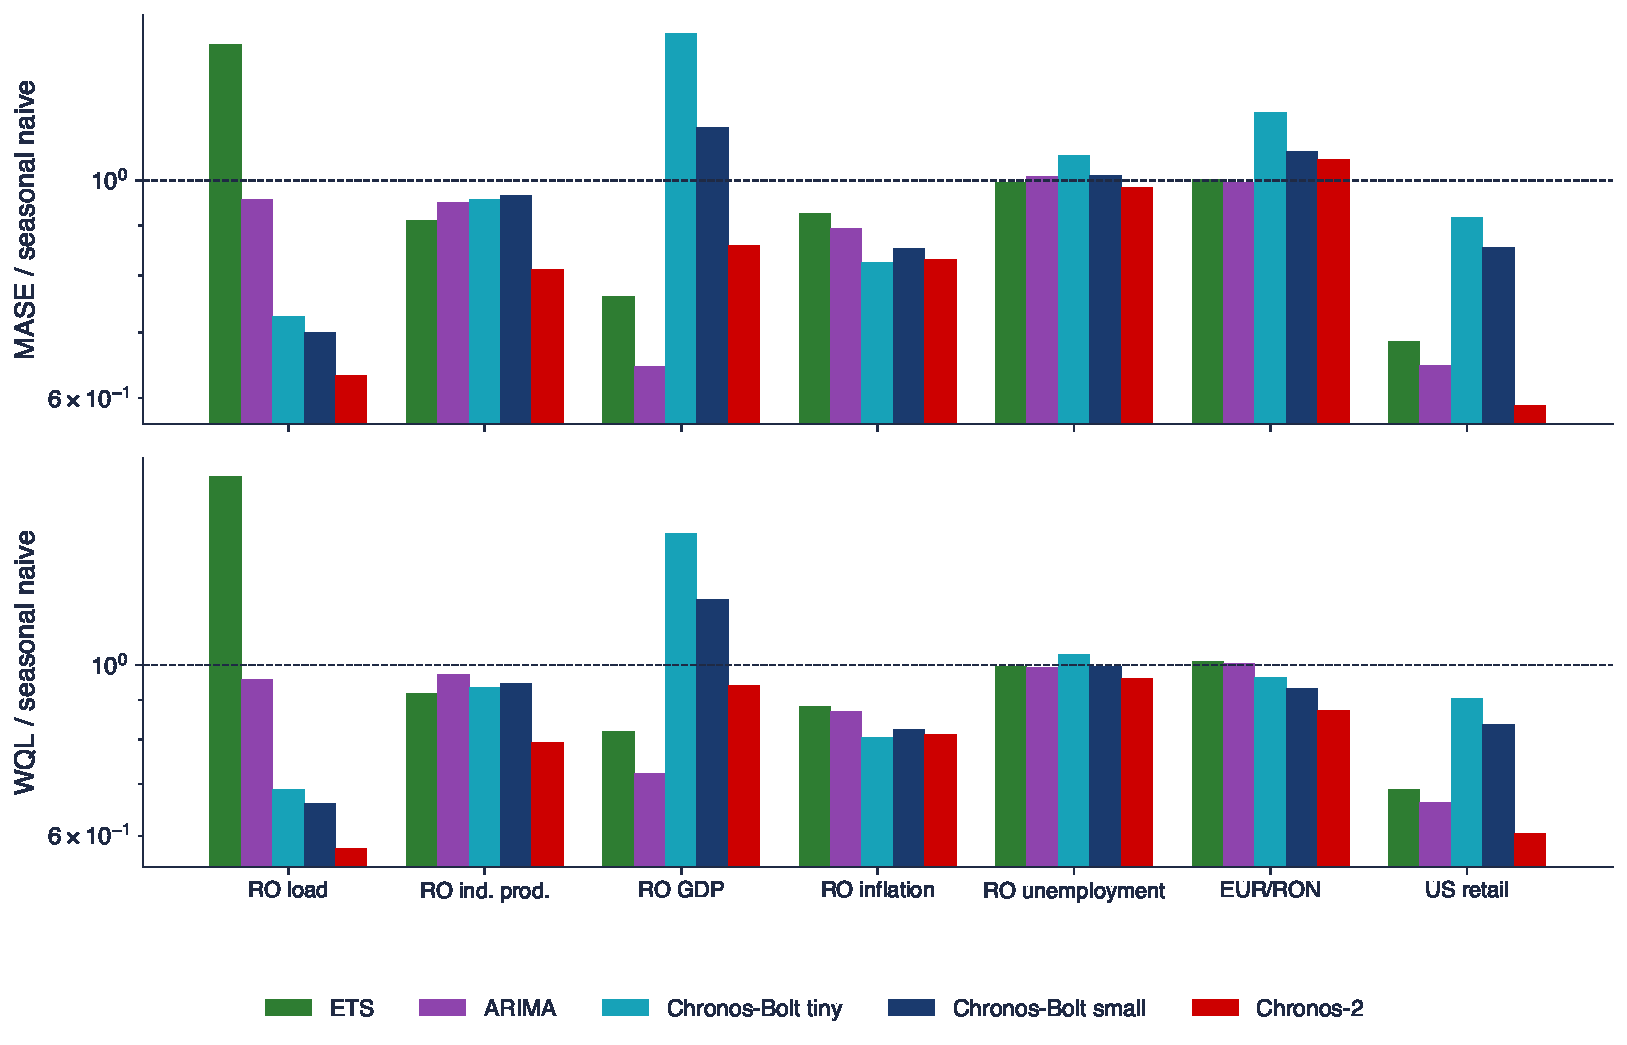
\includegraphics[width=0.97\textwidth,height=0.66\textheight,keepaspectratio]{tsa_ch11_benchmark.pdf}
\end{center}
\vspace{-0.25cm}
\begin{itemize}
    \item Ratios to the seasonal naive forecast (log scale; the dashed line is 1)
\end{itemize}
\quantlet{TSA\_ch11\_benchmark}{\qlurl{TSA_ch11_benchmark}}
\end{frame}

\begin{frame}{Interpreting the benchmark}
\itemsize{\footnotesize}
\begin{itemize}
    \item Hourly load: the foundation models win clearly (WQL ratio 0.58 for Chronos-2, 0.66 for Bolt small, 0.96 for ARIMA); ETS with a daily season only fails (1.75)
    \item Romanian GDP (short quarterly series): ARIMA is best (0.72); Chronos-Bolt is worse than the seasonal naive (1.22)
    \item Unemployment and EUR/RON: all models are close to 1: nothing beats the naive forecast by much
    \item Geometric mean of WQL: Chronos-2 0.78, ARIMA 0.87, Bolt small 0.90, Bolt tiny 0.95, ETS 0.97; Chronos-2 is best on 5 of 7 series
    \item A well-specified ARIMA is as good as the small foundation models; a single winner on all series does not exist
\end{itemize}
\end{frame}

\begin{frame}{Coverage of the 80\% intervals}
\itemsize{\footnotesize}
\begin{center}
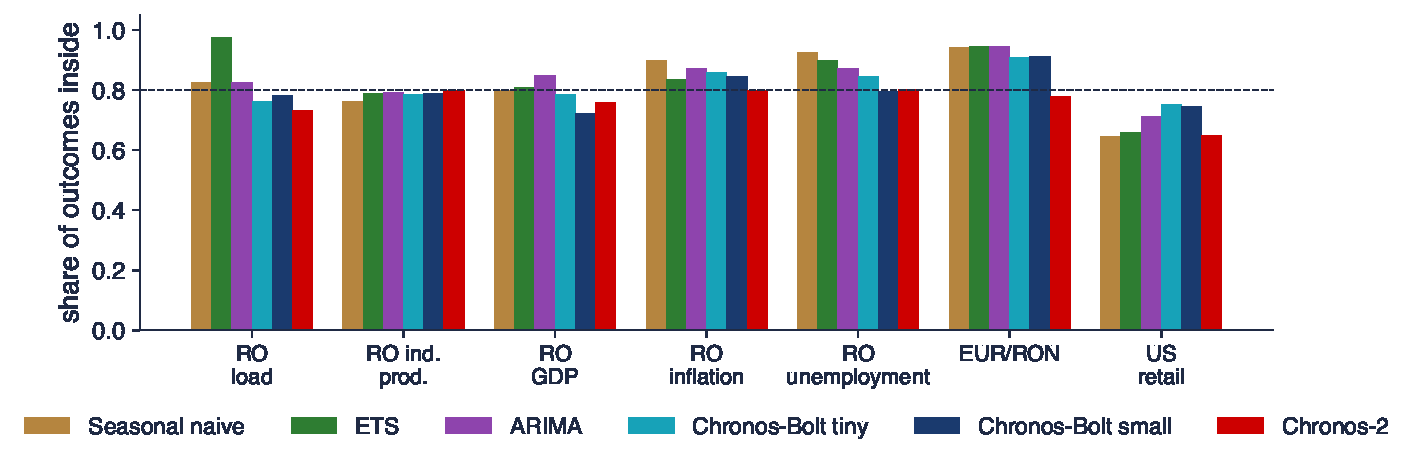
\includegraphics[width=0.97\textwidth,height=0.66\textheight,keepaspectratio]{tsa_ch11_coverage.pdf}
\end{center}
\vspace{-0.25cm}
\begin{itemize}
    \item Share of outcomes inside $[\hat q_{0.1}, \hat q_{0.9}]$, all origins and steps; the dashed line is the target 0.8
\end{itemize}
\quantlet{TSA\_ch11\_benchmark}{\qlurl{TSA_ch11_benchmark}}
\end{frame}

\begin{frame}{Interpreting the coverage}
\itemsize{\small}
\begin{itemize}
    \item Average coverage: seasonal naive 83\%, ETS 84\%, ARIMA 84\%, Bolt small 80\%, Chronos-2 76\%
    \item Chronos-2 has the best WQL but intervals that are too narrow: sharp, not fully calibrated
    \item US retail sales: every model covers well below 80\% (from 65\% for Chronos-2 to 75\% for Bolt tiny): the 2020 shock and the 2021 jump surprise all of them
    \item ETS and ARIMA bands assume Normal errors and constant variance: too wide in calm periods, too narrow in crises
\end{itemize}
\end{frame}

\begin{frame}{Romanian load: error by horizon}
\itemsize{\footnotesize}
\begin{center}
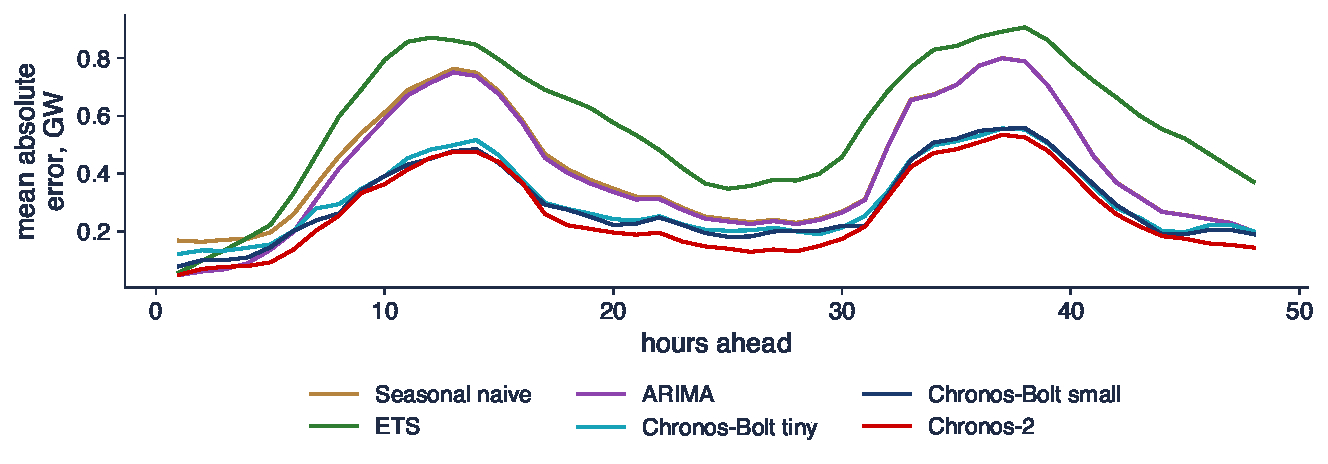
\includegraphics[width=0.97\textwidth,height=0.62\textheight,keepaspectratio]{tsa_ch11_horizon.pdf}
\end{center}
\vspace{-0.25cm}
\begin{itemize}
    \item Mean absolute error (GW) of the median forecast for each of the 48 hours ahead, over 52 weekly origins
\end{itemize}
\quantlet{TSA\_ch11\_benchmark}{\qlurl{TSA_ch11_benchmark}}
\end{frame}

\begin{frame}{Interpreting the error by horizon}
\itemsize{\small}
\begin{itemize}
    \item First hour: ARIMA 0.05 and Chronos-2 0.05 GW, far better than the seasonal naive 0.17: the last observation matters most
    \item After one day ARIMA is back to the naive level (0.24 against 0.25 GW): its correction fades out
    \item Chronos-2 keeps an advantage over the whole horizon (0.14 GW at 48 hours against 0.20)
    \item ETS is good for a few hours and then the worst: a daily season cannot represent the weekend
\end{itemize}
\end{frame}

\begin{frame}{How much context is needed? (1/2)}
\itemsize{\small}
\centering
\makebox[\textwidth][c]{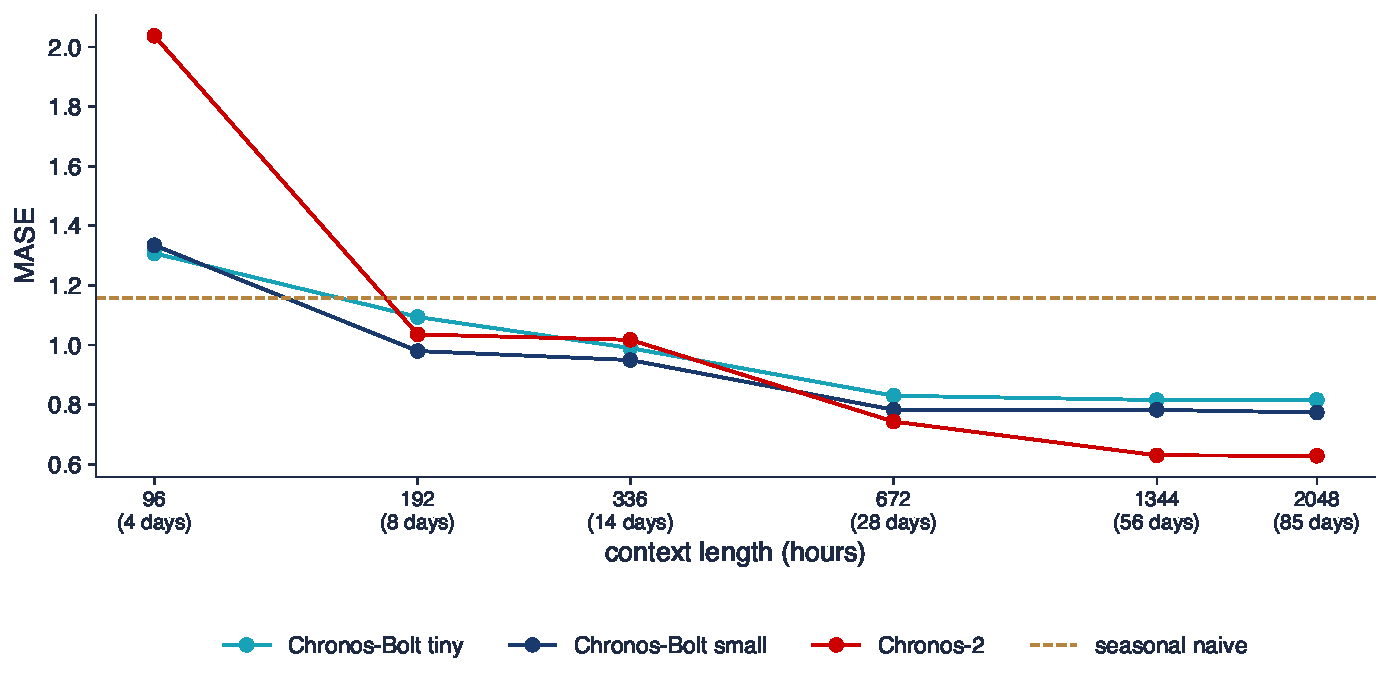
\includegraphics[width=0.96\paperwidth,height=0.88\textheight,keepaspectratio]{tsa_ch11_context.pdf}}
\end{frame}

\begin{frame}{How much context is needed? (2/2)}
\itemsize{\small}
\begin{itemize}
    \item MASE on Romanian load for contexts of 96 to 2048 hours; 26 weekly origins (the last half year); the dashed line is the seasonal naive
\end{itemize}
\quantlet{TSA\_ch11\_context\_contamination}{\qlurl{TSA_ch11_context_contamination}}
\end{frame}

\begin{frame}{Interpreting the context length}
\itemsize{\small}
\begin{itemize}
    \item With 96 hours (4 days) every model is worse than the seasonal naive: Chronos-Bolt small 1.33, Chronos-2 2.04, naive 1.16
    \item From 192 hours (more than one week) on, the weekly cycle is in the context and the error drops
    \item Chronos-2 keeps improving up to 1344 hours (0.63); Chronos-Bolt flattens at 672 hours (0.78)
    \item Rule: give the model several full seasonal cycles; a zero-shot model only repeats what it sees
\end{itemize}
\end{frame}

\begin{frame}{Size and accuracy}
\itemsize{\footnotesize}
\begin{center}
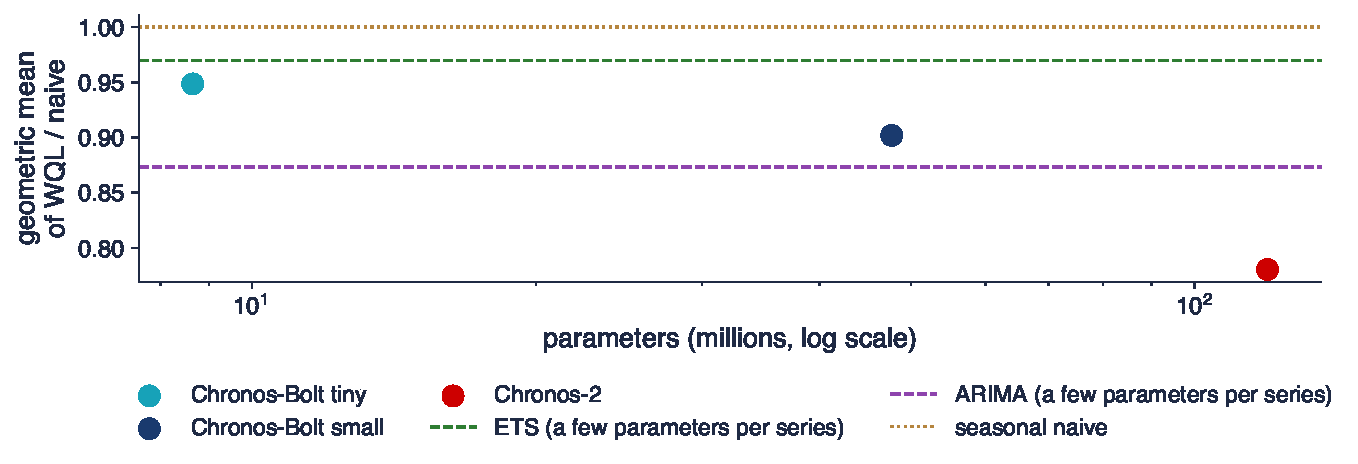
\includegraphics[width=0.97\textwidth,height=0.62\textheight,keepaspectratio]{tsa_ch11_size.pdf}
\end{center}
\vspace{-0.25cm}
\begin{itemize}
    \item Geometric mean over the seven series of the WQL ratio to the seasonal naive, against the number of parameters
\end{itemize}
\quantlet{TSA\_ch11\_context\_contamination}{\qlurl{TSA_ch11_context_contamination}}
\end{frame}

\begin{frame}{Interpreting size and cost}
\itemsize{\small}
\begin{itemize}
    \item Parameters: Bolt tiny 9 million, Bolt small 48 million, Chronos-2 119 million; ETS and ARIMA: a few per series
    \item Accuracy improves with size, but ARIMA (0.87) sits between the small and the large model
    \item Time per load forecast on a laptop CPU: Bolt small 19 ms, Chronos-2 43 ms, ARIMA 114 ms, ETS 411 ms
    \item Zero-shot inference is cheap; the cost was paid once, in pretraining
\end{itemize}
\end{frame}

\begin{frame}{Landmark benchmarks}
\itemsize{\footnotesize}
\begin{itemize}
    \item \textbf{M3} (\refMH)
    \begin{itemize}
        \item 3003 series
        \item sophisticated methods did not beat simple ones on average
    \end{itemize}
    \item \textbf{M4} (\refMSA)
    \begin{itemize}
        \item 100\,000 series
        \item combinations and a hybrid of exponential smoothing and a neural network won
    \end{itemize}
    \item \textbf{Monash archive} (\refMonash)
    \begin{itemize}
        \item public data sets with fixed horizons and benchmark results
    \end{itemize}
    \item \textbf{GIFT-Eval} (\refAksu)
    \begin{itemize}
        \item many domains and frequencies, MASE and CRPS, a public leaderboard of foundation models
        \item separates the test data from a pretraining corpus, to limit contamination
    \end{itemize}
    \item Critical studies: simple linear models beat early Transformer forecasters (\refZeng); LLM parts add no accuracy (\refTan)
\end{itemize}
\end{frame}

\begin{frame}{When foundation models help, and when not}
\itemsize{\footnotesize}
\begin{itemize}
    \item \textbf{Help}
    \begin{itemize}
        \item many series, little time per series; strong and regular seasonality; long contexts (load, sales, traffic)
        \item a quick, strong benchmark before building a dedicated model; probabilistic output at no extra cost
    \end{itemize}
    \item \textbf{Do not help}
    \begin{itemize}
        \item series close to a random walk (exchange rates, returns): nothing to learn from the past
        \item short series (a few dozen quarters) where a careful ARIMA is better
        \item when drivers matter (temperature, prices, policy) and are not in the context
        \item when the model must be explained parameter by parameter, or a causal question is asked
    \end{itemize}
    \item Always compare with seasonal naive, ETS and ARIMA on the same origins; test differences with Diebold--Mariano (\refDM)
\end{itemize}
\end{frame}

\begin{frame}{Recap: The evaluation}
\itemsize{\small}
\begin{itemize}
    \item Chronos-2 is best on average, especially for hourly load; ARIMA is close and wins on GDP
    \item On random-walk-like series no model beats the naive forecast
    \item Intervals of foundation models tend to be too narrow; context must cover the seasons
\end{itemize}
\end{frame}


%=============================================================================
\section{Leakage and contamination}
%=============================================================================

\begin{frame}{Leakage in your own pipeline}
\itemsize{\footnotesize}
\begin{itemize}
    \item \textbf{Leakage}
    \begin{itemize}
        \item information from the test period reaches the forecasts (\refHew)
    \end{itemize}
    \item Typical mistakes
    \begin{itemize}
        \item scaling or standardising with the mean of the whole sample
        \item choosing ARIMA orders, the context length or the model version after looking at test errors
        \item using revised data (GDP) as if it had been known at the origin
        \item random train/test splits of a time series (\tsachlink{https://danpele.github.io/Time-Series-Analysis/EN/Courses/chapter9_machine_learning_time_series.pdf}{Chapter 9})
    \end{itemize}
    \item In this chapter: each context ends at the origin; ARIMA orders were fixed before the first origin; Chronos scales by the context only
    \begin{itemize}
        \item remaining issue: Eurostat GDP and production are the latest vintage, not real-time data
    \end{itemize}
\end{itemize}
\end{frame}

\begin{frame}{Contamination of benchmarks}
\itemsize{\footnotesize}
\begin{itemize}
    \item \textbf{Contamination}
    \begin{itemize}
        \item the test series (or series highly correlated with it) were in the pretraining corpus
        \item the score then measures memory, not forecasting: an optimistic bias
    \end{itemize}
    \item Chronos reports two benchmarks: in-domain (data sets used in training) and zero-shot (data sets not used) (\refAnsari)
    \begin{itemize}
        \item public series such as M4 or US macro data are likely in many corpora; FRED is public, so is Eurostat
    \end{itemize}
    \item Remedies
    \begin{itemize}
        \item test only on data published after the release date of the weights
        \item live benchmarks: forecasts submitted before the outcome exists
        \item report the training corpus and the release date of every model you use
    \end{itemize}
\end{itemize}
\end{frame}

\begin{frame}{A contamination check: before and after the release}
\itemsize{\footnotesize}
\begin{center}
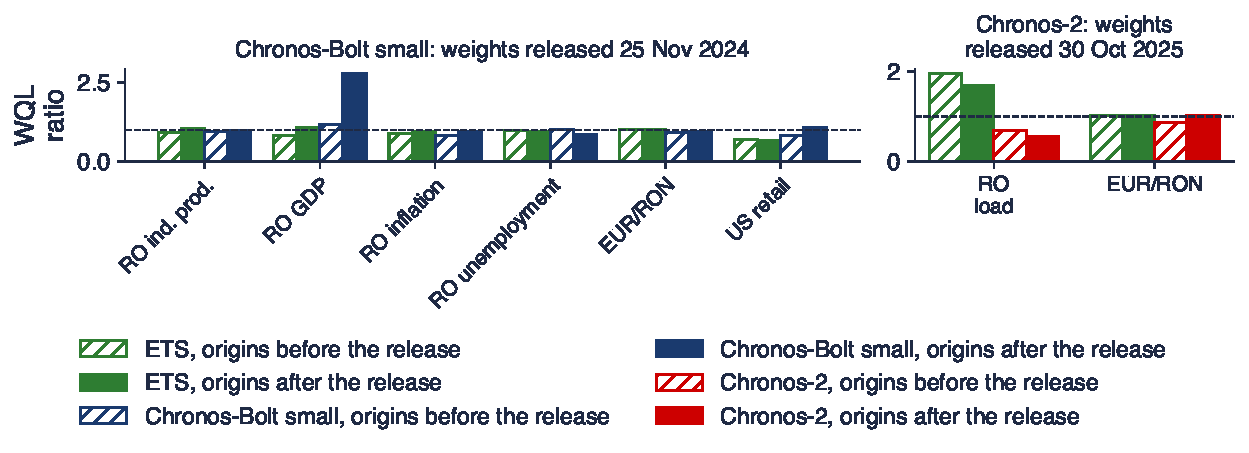
\includegraphics[width=0.97\textwidth,height=0.66\textheight,keepaspectratio]{tsa_ch11_prepost.pdf}
\end{center}
\vspace{-0.25cm}
\begin{itemize}
    \item WQL ratio to the seasonal naive for origins before (hatched) and after (solid) the release of the weights; ETS on the same origins as control
\end{itemize}
\quantlet{TSA\_ch11\_context\_contamination}{\qlurl{TSA_ch11_context_contamination}}
\end{frame}

\begin{frame}{Interpreting the contamination check}
\itemsize{\footnotesize}
\begin{itemize}
    \item Chronos-2 on EUR/RON: 0.86 before its release (124 origins), 1.02 after (10 origins): the advantage disappears
    \item Chronos-2 on load: 0.68 before, 0.54 after: the gain is real, also on data it could not have seen
    \item Chronos-Bolt small, US retail: 0.82 before, 1.08 after, while ETS is stable (0.69, 0.68)
    \item Caution: 3 to 35 origins after the release are few; the after period also differs (2025--2026); a drop is a warning, not a proof
    \item Chronos-2 was released in October 2025: its monthly results above use only origins before that date
\end{itemize}
\end{frame}

\begin{frame}{Recap: Leakage and contamination}
\itemsize{\small}
\begin{itemize}
    \item Leakage is under your control: use only data available at each origin
    \item Contamination is not: the pretraining corpus may contain your series
    \item Check results on data released after the model
\end{itemize}
\end{frame}


%=============================================================================
\section{Possible contribution of AI}
%=============================================================================

\begin{frame}{Possible contribution of AI}
\itemsize{\small}
\begin{itemize}
    \item \textbf{Code}
    \begin{itemize}
        \item a first draft of a rolling-origin backtest, of the pinball loss and the WQL, of a fan chart
    \end{itemize}
    \item \textbf{Reading}
    \begin{itemize}
        \item a summary of a model paper (architecture, corpus, licence, release date)
    \end{itemize}
    \item \textbf{Exploration}
    \begin{itemize}
        \item run several open models on many Romanian series from Eurostat or INS
    \end{itemize}
    \item Example prompt
    \begin{itemize}
        \item \aiprompt{Write Python code that downloads Romanian monthly industrial production (Eurostat sts\_inpr\_m, not seasonally adjusted), forecasts 12 months ahead from monthly origins since 2016 with amazon/chronos-bolt-small (package chronos-forecasting, CPU), ETS and the seasonal naive, and reports MASE, the weighted quantile loss and the coverage of the 80\% interval.}
    \end{itemize}
\end{itemize}
\end{frame}

\begin{frame}{Checks you must run}
\itemsize{\small}
\begin{itemize}
    \item The package and the model names: \texttt{BaseChronosPipeline}, \texttt{amazon/chronos-bolt-small}; an invented class or model name fails at once
    \item The context ends at the origin: no scaling, ordering or tuning with test data
    \item The quantile levels: Chronos-Bolt gives only 0.1 to 0.9; a ``1\% quantile'' from it is an extrapolation
    \item The benchmarks: seasonal naive, ETS and ARIMA on the same origins; scores relative to the naive forecast
    \item The release date of the weights against the test period; claims of ``state of the art'' need a source
    \item Every cited paper: it must exist; check the arXiv number or the DOI
\end{itemize}
\end{frame}


%=============================================================================
\section{Summary}
%=============================================================================

\begin{frame}{Key takeaways}
\itemsize{\small}
\begin{itemize}
    \item A foundation model is pretrained once on many series and forecasts new series zero-shot, from the context only
    \item Series become Transformer inputs by scaling, quantisation (Chronos) or patching (TimesFM, Moirai, Chronos-Bolt)
    \item Outputs are quantiles: score them with the pinball loss, the CRPS or WQL, and check coverage
    \item On our seven series: large gains on hourly load, none on random-walk-like series, losses on short quarterly GDP; ARIMA remains a strong benchmark
    \item Contamination can inflate published scores: test on data released after the model
\end{itemize}
\end{frame}

\begin{frame}{Key formulas}
\itemsize{\small}
{\renewcommand{\arraystretch}{1.4}\begin{center}
\footnotesize
\begin{tabular}{ll}
\toprule
\textbf{Quantity} & \textbf{Formula} \\
\midrule
Attention & $\text{softmax}(QK^\top/\sqrt{d})\,V$ \\
Mean scaling & $\tilde x_t = x_t/s$, \quad $s = \frac1C\sum_{t=1}^{C}|x_t|$ \\
Pinball loss & $L_\tau(y, \hat q_\tau) = \max\{\tau(y - \hat q_\tau),\ (\tau - 1)(y - \hat q_\tau)\}$ \\
CRPS & $\int (F(z) - \mathbf{1}\{z \ge y\})^2\,dz = 2\int_0^1 L_\tau(y, F^{-1}(\tau))\,d\tau$ \\
WQL & $\frac{1}{9}\sum_{\tau} 2\sum_t L_{\tau}(y_t, \hat q_{\tau,t}) \big/ \sum_t |y_t|$ \\
MASE & $\frac1h\sum_j |y_{T+j} - \hat y_{T+j}| \Big/ \frac{1}{T-m}\sum_{t>m}|y_t - y_{t-m}|$ \\
Coverage & $\frac1n\sum_i \mathbf{1}\{\hat q_{0.1}^{(i)} \le y_i \le \hat q_{0.9}^{(i)}\}$, target 0.8 \\
\bottomrule
\end{tabular}
\end{center}
}
\end{frame}

\begin{frame}{Self-assessment (1/2)}
\itemsize{\small}
\begin{itemize}
    \item \textbf{Question}: what is the difference between zero-shot forecasting and fine-tuning?
    \begin{itemize}
        \item \textbf{Answer}: zero-shot keeps the pretrained weights fixed and uses only the context; fine-tuning trains the weights further on the target data
    \end{itemize}
    \item \textbf{Question}: a context is 10, 20, 30. What are $s$ and the scaled values in Chronos?
    \begin{itemize}
        \item \textbf{Answer}: $s = 20$; scaled values 0.5, 1, 1.5
    \end{itemize}
    \item \textbf{Question}: $\hat q_{0.9} = 5$ and $y = 6$. What is the pinball loss?
    \begin{itemize}
        \item \textbf{Answer}: $0.9 \cdot (6 - 5) = 0.9$
    \end{itemize}
    \item \textbf{Question}: how many patches of 16 does a context of 512 values give?
    \begin{itemize}
        \item \textbf{Answer}: 32
    \end{itemize}
\end{itemize}
\end{frame}

\begin{frame}{Self-assessment (2/2)}
\itemsize{\small}
\begin{itemize}
    \item \textbf{Question}: an 80\% interval covers 95\% of the outcomes. Is this good?
    \begin{itemize}
        \item \textbf{Answer}: no: the intervals are too wide (not sharp); the CRPS penalises this
    \end{itemize}
    \item \textbf{Question}: why can a foundation model not beat the random walk on EUR/RON?
    \begin{itemize}
        \item \textbf{Answer}: the changes of the rate are close to unpredictable from the past; no model can extract information that the context does not contain
    \end{itemize}
    \item \textbf{Question}: a model released in 2025 scores very well on test data from 2018--2023. What do you check?
    \begin{itemize}
        \item \textbf{Answer}: whether those series were in its pretraining corpus; repeat the test on data published after the release
    \end{itemize}
    \item \textbf{Idea for a project}: compare Chronos-Bolt, Chronos-2 and ARIMA on all Romanian monthly series of one Eurostat data set, before and after the release dates
    \item Next: \tsachlink{https://danpele.github.io/Time-Series-Analysis/EN/Courses/chapter12_spectral_analysis.pdf}{Chapter 12}, spectral analysis
\end{itemize}
\end{frame}


%=============================================================================
\section{References}
%=============================================================================

\begin{frame}{References (1/3)}
\itemsize{\scriptsize}
\begin{itemize}
    \item Aksu, T., Woo, G., Liu, J., Liu, X., et al.\ (2024). GIFT-Eval: A benchmark for general time series forecasting model evaluation. \href{https://arxiv.org/abs/2410.10393}{arXiv:2410.10393}
    \item Ansari, A. F., Stella, L., Turkmen, C., Zhang, X., et al.\ (2024). Chronos: Learning the language of time series. \textit{Transactions on Machine Learning Research}. \href{https://arxiv.org/abs/2403.07815}{arXiv:2403.07815}
    \item Ansari, A. F., Shchur, O., Küken, J., Auer, A., et al.\ (2025). Chronos-2: From univariate to universal forecasting. \href{https://arxiv.org/abs/2510.15821}{arXiv:2510.15821}
    \item Bommasani, R., Hudson, D. A., Adeli, E., Altman, R., et al.\ (2021). On the opportunities and risks of foundation models. \href{https://arxiv.org/abs/2108.07258}{arXiv:2108.07258}
    \item Das, A., Kong, W., Sen, R., \& Zhou, Y. (2024). A decoder-only foundation model for time-series forecasting. \textit{Proceedings of the 41st International Conference on Machine Learning (ICML)}. \href{https://arxiv.org/abs/2310.10688}{arXiv:2310.10688}
    \item Diebold, F. X., \& Mariano, R. S. (1995). Comparing predictive accuracy. \textit{Journal of Business \& Economic Statistics}, 13(3), 253--263. \href{https://doi.org/10.1080/07350015.1995.10524599}{doi:10.1080/07350015.1995.10524599}
    \item Garza, A., Challu, C., \& Mergenthaler-Canseco, M. (2023). TimeGPT-1. \href{https://arxiv.org/abs/2310.03589}{arXiv:2310.03589}
    \item Gneiting, T., \& Raftery, A. E. (2007). Strictly proper scoring rules, prediction, and estimation. \textit{Journal of the American Statistical Association}, 102(477), 359--378. \href{https://doi.org/10.1198/016214506000001437}{doi:10.1198/016214506000001437}
\end{itemize}
\end{frame}

\begin{frame}{References (2/3)}
\itemsize{\scriptsize}
\begin{itemize}
    \item Godahewa, R., Bergmeir, C., Webb, G. I., Hyndman, R. J., \& Montero-Manso, P. (2021). Monash time series forecasting archive. \textit{NeurIPS Track on Datasets and Benchmarks}. \href{https://arxiv.org/abs/2105.06643}{arXiv:2105.06643}
    \item Gruver, N., Finzi, M., Qiu, S., \& Wilson, A. G. (2023). Large language models are zero-shot time series forecasters. \textit{Advances in Neural Information Processing Systems}, 36. \href{https://arxiv.org/abs/2310.07820}{arXiv:2310.07820}
    \item Hewamalage, H., Ackermann, K., \& Bergmeir, C. (2023). Forecast evaluation for data scientists: Common pitfalls and best practices. \textit{Data Mining and Knowledge Discovery}, 37(2), 788--832. \href{https://doi.org/10.1007/s10618-022-00894-5}{doi:10.1007/s10618-022-00894-5}
    \item Huang, C., \& Petukhina, A. (2022). \textit{Applied Time Series Analysis and Forecasting with Python}. Springer. \href{https://doi.org/10.1007/978-3-031-13584-2}{doi:10.1007/978-3-031-13584-2}
    \item Hyndman, R. J., \& Athanasopoulos, G. (2021). \textit{Forecasting: Principles and Practice} (3rd ed.). OTexts. \href{https://otexts.com/fpp3/}{otexts.com/fpp3}
    \item Hyndman, R. J., \& Koehler, A. B. (2006). Another look at measures of forecast accuracy. \textit{International Journal of Forecasting}, 22(4), 679--688. \href{https://doi.org/10.1016/j.ijforecast.2006.03.001}{doi:10.1016/j.ijforecast.2006.03.001}
    \item Makridakis, S., \& Hibon, M. (2000). The M3-Competition: Results, conclusions and implications. \textit{International Journal of Forecasting}, 16(4), 451--476. \href{https://doi.org/10.1016/S0169-2070(00)00057-1}{doi:10.1016/S0169-2070(00)00057-1}
    \item Makridakis, S., Spiliotis, E., \& Assimakopoulos, V. (2020). The M4 Competition: 100,000 time series and 61 forecasting methods. \textit{International Journal of Forecasting}, 36(1), 54--74. \href{https://doi.org/10.1016/j.ijforecast.2019.04.014}{doi:10.1016/j.ijforecast.2019.04.014}
\end{itemize}
\end{frame}

\begin{frame}{References (3/3)}
\itemsize{\scriptsize}
\begin{itemize}
    \item Matheson, J. E., \& Winkler, R. L. (1976). Scoring rules for continuous probability distributions. \textit{Management Science}, 22(10), 1087--1096. \href{https://doi.org/10.1287/mnsc.22.10.1087}{doi:10.1287/mnsc.22.10.1087}
    \item Nie, Y., Nguyen, N. H., Sinthong, P., \& Kalagnanam, J. (2023). A time series is worth 64 words: Long-term forecasting with Transformers. \textit{International Conference on Learning Representations (ICLR)}. \href{https://arxiv.org/abs/2211.14730}{arXiv:2211.14730}
    \item Rasul, K., Ashok, A., Williams, A. R., Ghonia, H., et al.\ (2023). Lag-Llama: Towards foundation models for probabilistic time series forecasting. \href{https://arxiv.org/abs/2310.08278}{arXiv:2310.08278}
    \item Salinas, D., Flunkert, V., Gasthaus, J., \& Januschowski, T. (2020). DeepAR: Probabilistic forecasting with autoregressive recurrent networks. \textit{International Journal of Forecasting}, 36(3), 1181--1191. \href{https://doi.org/10.1016/j.ijforecast.2019.07.001}{doi:10.1016/j.ijforecast.2019.07.001}
    \item Tan, M., Merrill, M. A., Gupta, V., Althoff, T., \& Hartvigsen, T. (2024). Are language models actually useful for time series forecasting? \textit{Advances in Neural Information Processing Systems}, 37. \href{https://arxiv.org/abs/2406.16964}{arXiv:2406.16964}
    \item Vaswani, A., Shazeer, N., Parmar, N., Uszkoreit, J., et al.\ (2017). Attention is all you need. \textit{Advances in Neural Information Processing Systems}, 30. \href{https://arxiv.org/abs/1706.03762}{arXiv:1706.03762}
    \item Woo, G., Liu, C., Kumar, A., Xiong, C., Savarese, S., \& Sahoo, D. (2024). Unified training of universal time series forecasting Transformers. \textit{Proceedings of the 41st International Conference on Machine Learning (ICML)}. \href{https://arxiv.org/abs/2402.02592}{arXiv:2402.02592}
    \item Zeng, A., Chen, M., Zhang, L., \& Xu, Q. (2023). Are Transformers effective for time series forecasting? \textit{Proceedings of the AAAI Conference on Artificial Intelligence}, 37(9), 11121--11128. \href{https://doi.org/10.1609/aaai.v37i9.26317}{doi:10.1609/aaai.v37i9.26317}
\end{itemize}
\end{frame}

\end{document}
